% Options for packages loaded elsewhere
% Options for packages loaded elsewhere
\PassOptionsToPackage{unicode}{hyperref}
\PassOptionsToPackage{hyphens}{url}
\PassOptionsToPackage{dvipsnames,svgnames,x11names}{xcolor}
%
\documentclass[
  letterpaper,
  DIV=11,
  numbers=noendperiod]{scrartcl}
\usepackage{xcolor}
\usepackage{amsmath,amssymb}
\setcounter{secnumdepth}{-\maxdimen} % remove section numbering
\usepackage{iftex}
\ifPDFTeX
  \usepackage[T1]{fontenc}
  \usepackage[utf8]{inputenc}
  \usepackage{textcomp} % provide euro and other symbols
\else % if luatex or xetex
  \usepackage{unicode-math} % this also loads fontspec
  \defaultfontfeatures{Scale=MatchLowercase}
  \defaultfontfeatures[\rmfamily]{Ligatures=TeX,Scale=1}
\fi
\usepackage{lmodern}
\ifPDFTeX\else
  % xetex/luatex font selection
\fi
% Use upquote if available, for straight quotes in verbatim environments
\IfFileExists{upquote.sty}{\usepackage{upquote}}{}
\IfFileExists{microtype.sty}{% use microtype if available
  \usepackage[]{microtype}
  \UseMicrotypeSet[protrusion]{basicmath} % disable protrusion for tt fonts
}{}
\makeatletter
\@ifundefined{KOMAClassName}{% if non-KOMA class
  \IfFileExists{parskip.sty}{%
    \usepackage{parskip}
  }{% else
    \setlength{\parindent}{0pt}
    \setlength{\parskip}{6pt plus 2pt minus 1pt}}
}{% if KOMA class
  \KOMAoptions{parskip=half}}
\makeatother
% Make \paragraph and \subparagraph free-standing
\makeatletter
\ifx\paragraph\undefined\else
  \let\oldparagraph\paragraph
  \renewcommand{\paragraph}{
    \@ifstar
      \xxxParagraphStar
      \xxxParagraphNoStar
  }
  \newcommand{\xxxParagraphStar}[1]{\oldparagraph*{#1}\mbox{}}
  \newcommand{\xxxParagraphNoStar}[1]{\oldparagraph{#1}\mbox{}}
\fi
\ifx\subparagraph\undefined\else
  \let\oldsubparagraph\subparagraph
  \renewcommand{\subparagraph}{
    \@ifstar
      \xxxSubParagraphStar
      \xxxSubParagraphNoStar
  }
  \newcommand{\xxxSubParagraphStar}[1]{\oldsubparagraph*{#1}\mbox{}}
  \newcommand{\xxxSubParagraphNoStar}[1]{\oldsubparagraph{#1}\mbox{}}
\fi
\makeatother


\usepackage{longtable,booktabs,array}
\usepackage{calc} % for calculating minipage widths
% Correct order of tables after \paragraph or \subparagraph
\usepackage{etoolbox}
\makeatletter
\patchcmd\longtable{\par}{\if@noskipsec\mbox{}\fi\par}{}{}
\makeatother
% Allow footnotes in longtable head/foot
\IfFileExists{footnotehyper.sty}{\usepackage{footnotehyper}}{\usepackage{footnote}}
\makesavenoteenv{longtable}
\usepackage{graphicx}
\makeatletter
\newsavebox\pandoc@box
\newcommand*\pandocbounded[1]{% scales image to fit in text height/width
  \sbox\pandoc@box{#1}%
  \Gscale@div\@tempa{\textheight}{\dimexpr\ht\pandoc@box+\dp\pandoc@box\relax}%
  \Gscale@div\@tempb{\linewidth}{\wd\pandoc@box}%
  \ifdim\@tempb\p@<\@tempa\p@\let\@tempa\@tempb\fi% select the smaller of both
  \ifdim\@tempa\p@<\p@\scalebox{\@tempa}{\usebox\pandoc@box}%
  \else\usebox{\pandoc@box}%
  \fi%
}
% Set default figure placement to htbp
\def\fps@figure{htbp}
\makeatother


% definitions for citeproc citations
\NewDocumentCommand\citeproctext{}{}
\NewDocumentCommand\citeproc{mm}{%
  \begingroup\def\citeproctext{#2}\cite{#1}\endgroup}
\makeatletter
 % allow citations to break across lines
 \let\@cite@ofmt\@firstofone
 % avoid brackets around text for \cite:
 \def\@biblabel#1{}
 \def\@cite#1#2{{#1\if@tempswa , #2\fi}}
\makeatother
\newlength{\cslhangindent}
\setlength{\cslhangindent}{1.5em}
\newlength{\csllabelwidth}
\setlength{\csllabelwidth}{3em}
\newenvironment{CSLReferences}[2] % #1 hanging-indent, #2 entry-spacing
 {\begin{list}{}{%
  \setlength{\itemindent}{0pt}
  \setlength{\leftmargin}{0pt}
  \setlength{\parsep}{0pt}
  % turn on hanging indent if param 1 is 1
  \ifodd #1
   \setlength{\leftmargin}{\cslhangindent}
   \setlength{\itemindent}{-1\cslhangindent}
  \fi
  % set entry spacing
  \setlength{\itemsep}{#2\baselineskip}}}
 {\end{list}}
\usepackage{calc}
\newcommand{\CSLBlock}[1]{\hfill\break\parbox[t]{\linewidth}{\strut\ignorespaces#1\strut}}
\newcommand{\CSLLeftMargin}[1]{\parbox[t]{\csllabelwidth}{\strut#1\strut}}
\newcommand{\CSLRightInline}[1]{\parbox[t]{\linewidth - \csllabelwidth}{\strut#1\strut}}
\newcommand{\CSLIndent}[1]{\hspace{\cslhangindent}#1}



\setlength{\emergencystretch}{3em} % prevent overfull lines

\providecommand{\tightlist}{%
  \setlength{\itemsep}{0pt}\setlength{\parskip}{0pt}}



 


\usepackage{float}
\usepackage{tabularray}
\usepackage[normalem]{ulem}
\usepackage{graphicx}
\usepackage{rotating}
\UseTblrLibrary{siunitx}
\NewTableCommand{\tinytableDefineColor}[3]{\definecolor{#1}{#2}{#3}}
\newcommand{\tinytableTabularrayUnderline}[1]{\underline{#1}}
\newcommand{\tinytableTabularrayStrikeout}[1]{\sout{#1}}
\KOMAoption{captions}{tableheading}
\makeatletter
\@ifpackageloaded{caption}{}{\usepackage{caption}}
\AtBeginDocument{%
\ifdefined\contentsname
  \renewcommand*\contentsname{Table of contents}
\else
  \newcommand\contentsname{Table of contents}
\fi
\ifdefined\listfigurename
  \renewcommand*\listfigurename{List of Figures}
\else
  \newcommand\listfigurename{List of Figures}
\fi
\ifdefined\listtablename
  \renewcommand*\listtablename{List of Tables}
\else
  \newcommand\listtablename{List of Tables}
\fi
\ifdefined\figurename
  \renewcommand*\figurename{Figure}
\else
  \newcommand\figurename{Figure}
\fi
\ifdefined\tablename
  \renewcommand*\tablename{Table}
\else
  \newcommand\tablename{Table}
\fi
}
\@ifpackageloaded{float}{}{\usepackage{float}}
\floatstyle{ruled}
\@ifundefined{c@chapter}{\newfloat{codelisting}{h}{lop}}{\newfloat{codelisting}{h}{lop}[chapter]}
\floatname{codelisting}{Listing}
\newcommand*\listoflistings{\listof{codelisting}{List of Listings}}
\makeatother
\makeatletter
\makeatother
\makeatletter
\@ifpackageloaded{caption}{}{\usepackage{caption}}
\@ifpackageloaded{subcaption}{}{\usepackage{subcaption}}
\makeatother
\usepackage{bookmark}
\IfFileExists{xurl.sty}{\usepackage{xurl}}{} % add URL line breaks if available
\urlstyle{same}
\hypersetup{
  pdftitle={Do marine protected area announcements trigger preemptive overfishing? New insights from tuna catch and effort data},
  pdfauthor={Emily Rodriguez},
  colorlinks=true,
  linkcolor={blue},
  filecolor={Maroon},
  citecolor={Blue},
  urlcolor={Blue},
  pdfcreator={LaTeX via pandoc}}


\title{Do marine protected area announcements trigger preemptive
overfishing? New insights from tuna catch and effort data}
\author{Emily Rodriguez}
\date{}
\begin{document}
\maketitle
\begin{abstract}
Marine protected area (MPA) announcements have been cited as having the
potential to inadvertently increase fishing effort before closures are
implemented, a phenomenon known as the ``blue paradox''. The only known
evidence of a blue paradox comes from the Phoenix Island Protected Area
(PIPA), although some have contended that this event was driven by
environmental conditions shifting the location of tuna, rather than
preemptive fishing behavior. Using publicly available catch and effort
data, we ask whether previously reported increases in fishing effort are
due to anticipatory behavior or favorable environmental conditions. We
then ask whether the blue paradox is detectable for other large-scale
MPAs in the region. Our study makes three contributions. First, we find
no conclusive evidence whether the increase in fishing effort within
PIPA was driven by anticipatory behavior or environmental factors.
Second, we fail to detect evidence of a blue paradox in the other three
large-scale MPAs examined. And third, our study highlights that RFMO
data can be used for evaluating fishing dynamics across time periods
where vessel-tracking data, which became widely accessible in 2018, were
unavailable.
\end{abstract}


\textbf{Keywords}: Blue Paradox, Marine Protected Areas, Fishing
Behavior, Fisheries Management, Overfishing

\section{Introduction}\label{introduction}

The recently signed Kunming-Montreal Global Biodiversity ``30x30''
target (Target 3) calls for at least 30\% of marine regions to be
effectively conserved or managed by 2030 using marine protected areas
(MPAs) and other area-based conservation measures (Secretariat of the
Convention on Biological Diversity 2022). Importantly, Target 3 also
mentions that the establishment and management of protected areas should
involve relevant actors in local communities to ensure transparency,
participation, and resilient management. However, early disclosure of
MPAs could create a tension: informing fishers in advance may encourage
preemptive exploitation of resources, potentially undermining
conservation objectives. McDermott et al. (2019) termed this phenomenon
the ``blue paradox'' after documenting a surge in fishing effort in the
months leading up to the implementation of the Phoenix Islands Protected
Area (PIPA) in Kiribati, an important region for industrial tuna fishing
(Hernández et al. 2019). As the global coverage of protected regions
expand, the timing and communication of MPA establishment may therefore
have increasingly important consequences for fishing behavior. Clearly,
a rising question for marine conservation is whether the announcement of
a marine protected area can unintentionally increase fishing effort
before protection begins.

One explanation for anticipatory fishing behavior comes from
psychological reactance, which suggests that people resist perceived
threats to their freedom by attempting to restore it (Brehm 1966). The
restriction-sensitive choice model builds on this idea by formalizing
how removing or restricting options can paradoxically make them more
desirable (Boissonnet and Ghersengorin 2025). A related phenomenon
appears in environmental regulation, where anticipated restrictions
induced individuals to eliminate the very conditions that would trigger
those restrictions. For example, in the case of the red-cockaded
woodpecker, research found that private forest owners in North Carolina
preemptively destroyed the endangered species' habitat by prematurely
harvesting trees to avoid the species inhabiting their property. In
turn, landowners prevented regulations on their property that would have
been imposed by the Endangered Species Act. This preemptive behavior
ultimately reduced the critical habitat that the listing of the species
intended to protect, illustrating how anticipated regulations can
trigger counterproductive or defensive actions (Lueck and Michael 2000).
This example suggests that under some circumstances, conservation
policies can unintentionally alter behavior before restrictions take
effect, providing a theoretical framework for interpreting the blue
paradox.

Given the growing call for MPA implementation, it is critical to
consider how MPA announcements impact fishing effort in
soon-to-be-protected grounds. McDermott et al. (2019) reported that the
announcement of the future no-take MPA, PIPA (Figure~\ref{fig-aoi}),
triggered a surge in fishing effort within the area slated for
protection prior to its establishment. The recorded fishing effort was
estimated to be equivalent to 1.5 years of banned fishing. Two competing
explanations have been proposed for the observed increase in fishing
effort. McDermott et al. (2019) interpreted the increase as an
anticipatory behavioral response to the announced closure (blue
paradox). Under this hypothesis, fishing effort increases on a stock
size that remains constant. Assuming catchability (\(q\)) remains
constant, the relationship \(\text{CPUE} = qN\) predicts that catch per
unit effort (CPUE) should remain \emph{constant} or even later decrease
if stock numbers are depleted. In contrast, Hanich et al. (2018) argued
that the El Niño Southern Oscillation (ENSO) during the time of the
study elevated tuna abundance in the region, consistent with evidence
linking ENSO conditions to changes in tuna abundance and distribution
(Lehodey et al. 1997). This increase in abundance, they argued,
contributed to a rise in purse seine effort within the Central Pacific
region from 19.8\% in 2014 to 31.4\% in 2015 (Hanich et al. 2018). By
their argument, the increase in fishing effort is driven by an increase
in tuna abundance. If biomass (\(N\)) increased and catchability (\(q\))
remained constant while fishing effort increased, CPUE would be expected
to \emph{increase} across the soon-to-be MPA.

\begin{figure}

\centering{

\pandocbounded{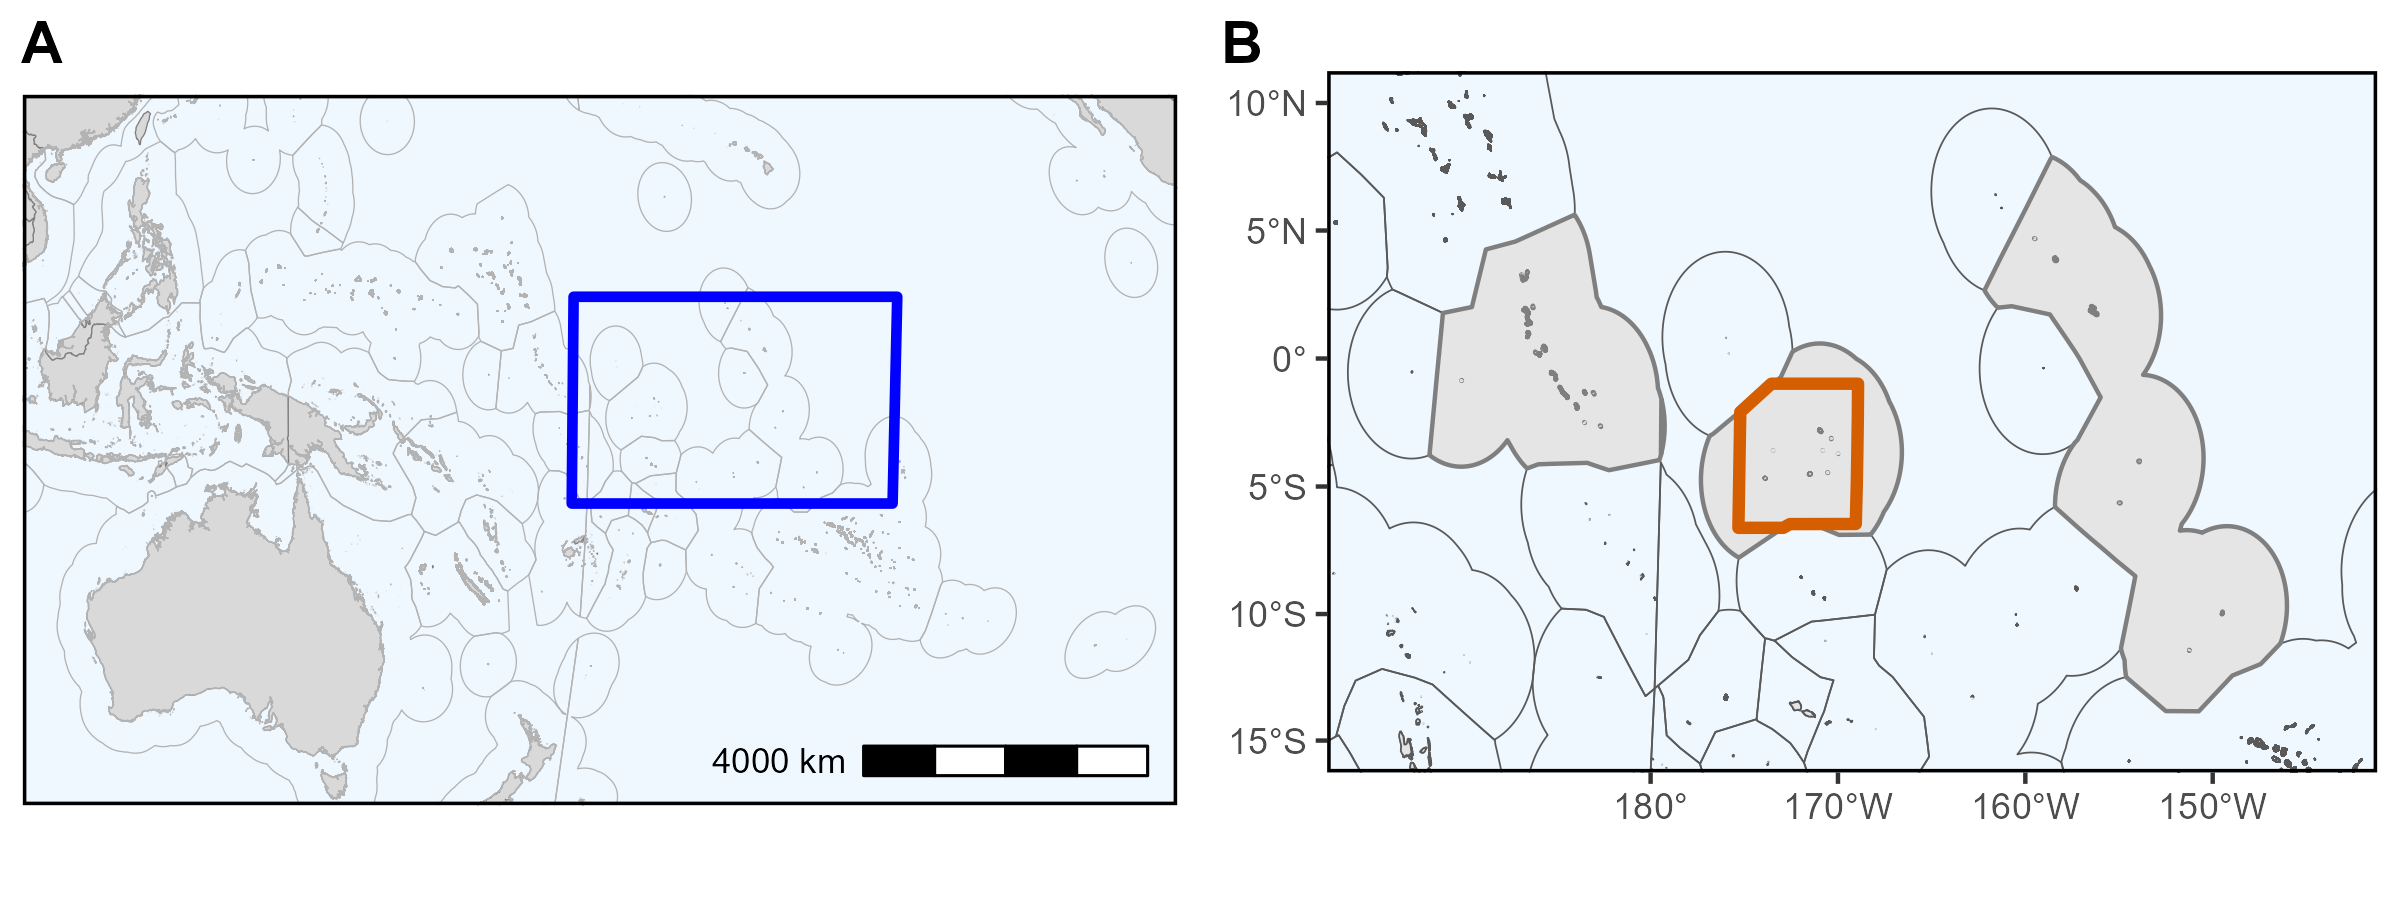
\includegraphics[keepaspectratio]{../results/figures/pipa_original/map_studyarea.png}}

}

\caption[Geographic context of the Phoenix Islands Protected
Area]{\label{fig-aoi}(A) Location of the Kiribati Islands denoted by the
blue outline relative to surrounding Exclusive Economic Zones (EEZs).
(B) Map of Kiribati Islands and respective EEZs. The Phoenix Islands
Protected Area is highlighted in red.}

\end{figure}%

The existing evaluation of the blue paradox relied only on fishing
effort derived from automatic identification system (AIS)
vessel-tracking data. It is important to note, however, that fishing
effort alone cannot distinguish whether increased activity reflects a
behavioral response by fishers or changing ecological conditions. In
order to reevaluate the potential blue paradox reported for PIPA, this
study makes three contributions. First, we assess whether the patterns
previously reported for PIPA using Global Fishing Watch's (GFW)
AIS-derived fishing effort data (Kroodsma et al. 2018) can be reproduced
using catch and effort data made publicly available by tuna Regional
Fisheries Management Organizations (RFMOs). Second, we extend the
previous analysis by incorporating catch data to calculate CPUE, an
imperfect proxy for local abundance (Maunder et al. 2006). These data
therefore allow us to distinguish changes in fishing effort from changes
in fish abundance. Third, we extend the blue paradox test to other
large-scale MPAs in the Pacific Ocean, including some implemented before
AIS data were available: Galápagos Marine Reserve (GMR) in Ecuador,
Revillagigedo National Park (RNP) in Mexico, and Palau National Marine
Sanctuary (PNMS) in Palau.

\section{Methods}\label{methods}

\subsection{Overview}\label{overview}

We begin with an evaluation of changes in fishing effort, catch, and
CPUE for the Phoenix Islands Protected Area. To distinguish a behavioral
response to the announced MPA, we use the same
Before-After-Control-Impact (BACI) framework introduced by McDermott et
al. (2019). The analysis compares fishing effort between the area within
the boundaries of the future MPA and comparable control areas outside
the MPA across before/after periods defined relative to the announcement
and implementation dates of the MPA. Additionally, we use catch and
effort data to assess changes in CPUE in order to distinguish the
predictions made by the blue paradox versus the environmental conditions
hypothesis. We specifically use commercial tuna purse seine data, as
this an important fishery in the region (Hernández et al. (2019)).

McDermott et al. (2019) previously analyzed fishing responses to the
PIPA announcement using GFW's daily fishing effort estimates aggregated
at the region level, measured in fishing hours per 1,000 km\(^2\). Our
approach differs in two ways. First, we deviate in that we measure
effort at the monthly level in fishing days or sets per 10,000 km\(^2\).
We them compliment the analysis by including catch data measured in
kilograms per 10,000 km\(^2\) to calculate CPUE per fishing day and set.

\subsection{Data sources}\label{data-sources}

This study uses publicly available data from RFMOs. The primary sources
are the Inter-American Tropical Tuna Commission (IATTC) and the Western
and Central Pacific Fisheries Commission (WCPFC) (Inter-American
Tropical Tuna Commission (2026), Western and Central Pacific Fisheries
Commission (2026)). Both RFMOs provide monthly purse seine catch and
effort data at a 1\(^\circ\) × 1\(^\circ\) spatial resolution, albeit
with some variation in their reporting standards. The data from each
RFMO were harmonized into a singular dataset used for this study
(Rodriguez and Juan Carlos Villaseñor-Derbez 2026). For each grid cell
and month, these data report the effort (days or sets) and total catch
(mt) of four main tuna species (\emph{Thunnus alalunga}, \emph{Thunnus
obesus}, \emph{Katsuwonus pelamis}, and \emph{Thunnus albacares}) caught
by purse seine fleets in the region. From these, CPUE was calculated in
mt/day and mt/set.

Vector files with polygons for PIPA, GMR, RNP, and the related EEZs were
obtained from the mregions2 R package (Guevara, Fernández Bejarano, and
Pohl 2024). Spatial data for the original 2015 PNMS were obtained from
UNEP-WCMC and IUCN (2026). Global country boundaries were obtained as a
spatial vector layer using the rnaturalearth package version 1.2.0
(Massicotte and South 2017).

\subsection{Data processing}\label{data-processing}

The BACI design requires that we identify before and after periods.
Temporal cutoffs were defined using the announcement and implementation
of each MPA. For PIPA, these dates followed the definitions established
by McDermott et al. (2019) in order to replicate the prior analysis: the
announcement date was defined as September 1, 2013, while the date of
implementation was defined as January 1, 2015.

The 1\(^\circ\) × 1\(^\circ\) spatial coordinates were extracted from
the RFMO data and rasterized. Spatial boundaries of PIPA and the related
Exclusive Economic Zones (EEZs) were then used to define cells into two
categories. Treated cells are those that lie inside or intersect with
the PIPA boundary. Control cells are those that lie inside or intersect
with either the Line Islands EEZ or the Gilbert Islands EEZ, the same
two control regions defined by McDermott et al. (2019). Cells that
partially intersected PIPA, even if they overlapped into the un-closed
surrounding EEZ of the Phoenix Islands, were retained to capture all
activity that might have happened inside the MPA. The same spatial
filtering method was used for the control region. The total extent of
PIPA, Line Islands EEZ, and Gilbert Islands EEZ were calculated in
km\(^2\), which we then used to normalize our outcomes of interest:
fishing effort (days per 10,000 km\(^2\) and sets per 10,000 km\(^2\)),
catch (kg per 10,000 km\(^2\)), and CPUE.

For each region and month, total effort (days and sets) and total catch
were calculated by summing observations across all fishing events. These
region-by-month totals were used as the outcome variables in the models.
The unit of observation is the region polygon, observed repeatedly
across months. Catch was converted from metric tons to kilograms to
improve model variable interpretation. CPUE was then calculated as the
ratio of total catch to total fishing effort, rather than aggregating
observation-level CPUE values. To account for differences in region
size, total fishing effort and total catch were standardized by region
area and expressed per 10,000 km\(^2\). The panel dataset includes
observations for the treated and control cells, the months before
implementation, and a treatment indicator (equal to 1 for cells within
for PIPA). The spatial distribution of fishing observations within the
treated and control regions are shown in Figure~\ref{fig-pipa-map}, with
a total of 203 observation points (N = 171 for the control region; N =
32 for the treated region). The resulting dataset contains 52 rows, with
28 observations from the control and 24 observations from the treated
region (Figure~\ref{fig-pipa-map}).

\subsection{Testing for a blue
paradox}\label{testing-for-a-blue-paradox}

We test for preemptive changes in fishing behavior via a multiple linear
regression model with the form:

\[\text{log}(Y_{it}) = \beta_0 + \beta_1\text{Treatment}_i + \beta_2\text{Post}_t + \beta_3(\text{Treatment}_i \times \text{Post}_t) + \epsilon_{it}\]

where \(Y_{it}\) is the outcome (effort per 10,000 km\(^2\), catch per
10,000 km\(^2\), or CPUE) in region \(i\) during month \(t\). Variables
\(\text{Treatment}_i\) and \(\text{Post}_t\) are indicator variables.
\(\text{Treatment}_i\) equals 1 for the treated region and 0 for the
control region. Similarly, \(\text{Post}_t\) equals 1 for months during
the anticipation period and 0 for months before the announcement. The
coefficient \(\beta_0\) is the intercept, representing the mean log
outcome for the control region before the announcement. Then,
\(\beta_1\) measures the mean difference in the log outcome between
treatment and control regions before the announcement, while \(\beta_2\)
measures the mean change in the log outcome over time for the control
region. Finally, \(\text{Treatment}_i \times \text{Post}_t\) is the
interaction term capturing the additional mean change in the log outcome
for the treated region during the anticipation period relative to the
mean change observed in the control region (blue paradox effect).
\(\epsilon_{it}\) is the error term.

Coefficients from the log-linear models were exponentiated in the
results to express effects as percentage changes. Percentage change was
calculated as \((e^{\beta}-1) \times 100\), where \(\beta\) represents
the estimated regression coefficient. This provides the exact percentage
change associated with a one-unit change in the predictor.

\subsection{Additional case studies}\label{additional-case-studies}

We extend the blue paradox to test three other MPAs: Galápagos Marine
Reserve (GMR) in Ecuador, Revillagigedo National Park (RNP) in Mexico,
and Palau National Marine Sanctuary (PNMS) in Palau. For each additional
case study, MPA announcement and implementation dates were defined using
available evidence as follows (Table~\ref{tbl-mpa-dates}).

The announcement date for GMR was defined as March 19, 1998, when GMR
was signed into law ({``Galápagos {Marine Reserve Celebrates} 25 {Years}
of {Creation}''} 2023). The definition for ``announcement'' was changed
here due to illegal fishing continuing in the region despite formal
implementation. Thus, the ``implementation'' date for GMR was defined as
January 1, 2002, corresponding to the date enforcement was added to the
MPA region (Boerder, Bryndum-Buchholz, and Worm 2017). We follow
Boerder, Bryndum-Buchholz, and Worm (2017) in adopting this enforcement
implementation date because their study focused on tuna fisheries within
the GMR, which are also the focus of our analysis. No specific
month-date was found for the GMR enforcement, so January 1 is assumed as
the month-start of enforcement in 2002.

For RNP, the announcement date was defined as October 5, 2017, based on
Naturales (2017), and the implementation date as November 27, 2017,
based on Martinez et al. (2025). The PNMS announcement date was defined
as October 22, 2015 (Martinez et al. 2025). Because PNMS was established
over a five-year period ({``Palau to {Sign National Marine Sanctuary
Into Law}''} (2015)), the implementation date was defined as the end of
the period on January 1, 2020 (Martinez et al. 2025). Fishing behavior
was analyzed one year prior to the announcement date.

Spatial processing rules to clip RFMO data to the treated and control
region were kept the same for each of the additional case studies.
Related EEZs were selected as the control region for all analyses to
similarly follow the selection criteria determined by McDermott et al.
(2019). For GMR, the control region was established as the mainland EEZ
of Ecuador (Figure~\ref{fig-gmr-map}). The Galápagos EEZ was not used as
a control region because the 1\(^\circ\) × 1\(^\circ\) spatial
resolution resulted in a limited number of independent observations.
Further more, several grid cells overlapped into GMR, reducing the
independence of the control region. The control region for RNP was
established as cells within 200 nautical miles of the MPA and within
Mexico's EEZ (Figure~\ref{fig-revilla-map}). Lastly, the PNMS treated
region was defined as the original 2015 boundary of the MPA (Jaiteh et
al. 2021). The control region for PNMS was established as cells within a
200 nautical mile region of Palau but within the Federated States of
Micronesia EEZ (Figure~\ref{fig-palau-map}). This approach was necessary
because the number of remaining observations in Palau was not sufficient
to support the analysis. The Federated States of Micronesia provides a
suitable comparison region due to its geographic proximity.
Additionally, both countries are signatories to the Parties to the Nauru
Agreement, and therefore operate under the same regional framework and
licensing mechanisms related to tuna fishing, making this a comparable
control region (Bernadett (2014)).

GMR was modeled the same as PIPA, but complete analyses for RNP and PNMS
were not possible due to limited data coverage. Additionally, GMR and
RNP lie within IATTC, who only report effort in sets. Therefore, effort
in days per 10,000 km\(^2\) and CPUE in kg/day were unavailable to be
tested.

\subsection{Processing}\label{processing}

All processing and analyses were conducted in R version 4.5.1 (R Core
Team 2025). Models were fit using the fixest package (version 0.14.0)
(Bergé, Butts, and McDermott 2026). Model tables were built using the
modelsummary package (version 2.6.0) (Vincent Arel-Bundock 2022) and
figures were created using ggplot2 (version 4.0.2)(Wickham 2016). Maps
were built using ggplot2 (Wickham 2016), rnaturalearth (version 1.2.0)
(Massicotte and South 2017) and sf (version 1.1.0)(Pebesma 2018).

\section{Results}\label{results}

\subsection{PIPA}\label{pipa}

Before evaluating treatment effects, we first compared estimates of
fishing activity derived from RFMO data and those derived from GFW data.
Monthly fishing effort time series comparing the datasets showed similar
patterns recorded a year prior to PIPA's announcement and leading up to
the MPA's implementation(Figure~\ref{fig-pipa-gfw-rfmo-days} and
Figure~\ref{fig-pipa-gfw-rfmo-days-hours}). These results demonstrate
that RFMO catch and effort records are a suitable basis for extending
previous evaluations of the blue paradox beyond fishing effort alone.

To characterize how fishing activity changed around the announcement of
PIPA, we examined time-series trends in effort, CPUE, and catch in the
control and treated regions (Figure~\ref{fig-pipa-region}). Across all
five outcomes, the control and treated regions exhibited broadly similar
temporal patterns prior to the announcement. Following the announcement
of PIPA, our results show an increase for both fishing effort in days
and sets per 10,000 km\(^2\) in the control region (Panels A-B). This
increase is accompanied by a corresponding rise in catch in kg per
10,000 km\(^2\) in the control region (Panel E). In contrast, effort and
catch in the treated region show slightly higher increases relative to
the control region, though not significant
(Table~\ref{tbl-pipa-region}). Across both regions, CPUE remains
relatively stable after the announcement date, with no clear shifts in
either kg/day or kg/set (Panels C-D).

Consistent with these visual patterns, the BACI interaction terms
indicate moderate, positive announcement effects in the treated region
relative to the control, though none of these estimates are
statistically significant (Table~\ref{tbl-pipa-region}). Specifically,
the announcement was associated with an increase in effort measured in
days and sets per 10,000 km \(^2\) (\(\beta\) = 0.336, SE = 0.656,
\emph{p} \textless{} 0.1; \(\beta\) = 0.354, SE = 0.692). Catch
increased with the announcement by 46.81\% within the treated region
relative to the changes observed in control region (\(\beta\) = 0.384,
SE = 0.678, \emph{p} \textless{} 0.1). However, CPUE in kg per days and
sets had minimal increase relative to the control region (\(\beta\) =
0.048, SE = 0.192, \emph{p} \textless{} 0.1; \(\beta\) = 0.030, SE =
0.181, \emph{p} \textless{} 0.1)(Table~\ref{tbl-pipa-region}).

We include robustness test in the supplementary content where we change
the definition of how pixels are assigned to treatment and controls.
This regression table provides a robustness check to match
Table~\ref{tbl-pipa-region} (Table~\ref{tbl-pipa-region_robust}). Here,
we restrict the treated region data to include only cells that are full
contained within PIPA. Our results show similar non-significant trends.

\begin{figure}

\centering{

\pandocbounded{\includegraphics[keepaspectratio]{../results/figures/pipa_original/cubic_timeseries_panels_region.png}}

}

\caption[Temporal trends in fishing effort, catch, and CPUE in the
Phoenix Islands Protected Area]{\label{fig-pipa-region}Cubic spline
estimates of temporal trends in five outcomes of interest for control
and treatment regions in the Phoenix Islands Protected Area (PIPA) at
the region-month level. Panels show observed monthly values (points) and
fitted cubic spline trajectories (lines) with shaded ribbons indicating
±1 standard error around the predicted values for (A) effort
(days/10,000 km\(^2\)), (B) effort (sets/10,000 km\(^2\)), (C) CPUE
(kg/day), (D) CPUE (kg/sets), and (E) total catch (kg/10,000 km\(^2\))
from September 2012 to December 2014. Panel F shows the treatment (PIPA)
and control regions. The vertical line indicates the announcement of
PIPA (2013-09-01). Data include all observations prior to MPA
implementation on 2015-01-01, with no post-implementation observations.}

\end{figure}%

\begin{table}

\caption{\label{tbl-pipa-region}Log-linear BACI regression estimates at
the region-level for Phoenix Islands Protected Area.}

\centering{

\centering
\begin{talltblr}[         %% tabularray outer open
caption={Log-linear BACI regression estimates at the region-level for Phoenix Islands Protected Area. The interaction term estimates the percentage change in the treatment region relative to the control region during the anticipation period.},
note{}={+ p \num{< 0.1}, * p \num{< 0.05}, ** p \num{< 0.01}, *** p \num{< 0.001}},
]                     %% tabularray outer close
{                     %% tabularray inner open
width={1\linewidth},
colspec={X[]X[]X[]X[]X[]X[]},
hline{2}={1-6}{solid, black, 0.05em},
hline{10}={1-6}{solid, black, 0.05em},
hline{1}={1-6}{solid, black, 0.08em},
hline{13}={1-6}{solid, black, 0.08em},
column{2-6}={}{halign=c},
column{1}={}{halign=l},
}                     %% tabularray inner close
& log Effort (days) / 10,000 km² & log Effort (sets) / 10,000 km² & log Total Catch (kg) / 10,000 km² & CPUE (kg/day) & CPUE (kg/set) \\
(Intercept) & \num{-0.001} & \num{0.044} & \num{10.295}*** & \num{10.296}*** & \num{10.251}*** \\
& (\num{0.328}) & (\num{0.346}) & (\num{0.339}) & (\num{0.096}) & (\num{0.091}) \\
treatment & \num{-0.025} & \num{-0.044} & \num{0.110} & \num{0.135} & \num{0.154} \\
& (\num{0.518}) & (\num{0.547}) & (\num{0.536}) & (\num{0.152}) & (\num{0.143}) \\
post & \num{1.328}** & \num{1.413}** & \num{1.390}** & \num{0.062} & \num{-0.023} \\
& (\num{0.434}) & (\num{0.458}) & (\num{0.448}) & (\num{0.127}) & (\num{0.120}) \\
treatment × post & \num{0.336} & \num{0.354} & \num{0.384} & \num{0.048} & \num{0.030} \\
& (\num{0.656}) & (\num{0.692}) & (\num{0.678}) & (\num{0.192}) & (\num{0.181}) \\
Num.Obs. & \num{52} & \num{52} & \num{52} & \num{52} & \num{52} \\
R2 & \num{0.313} & \num{0.315} & \num{0.334} & \num{0.082} & \num{0.075} \\
R2 Adj. & \num{0.270} & \num{0.272} & \num{0.293} & \num{0.025} & \num{0.017} \\
\end{talltblr}

}

\end{table}%

\subsection{Additional case studies}\label{additional-case-studies-1}

We have shown that RFMO data can capture the same broad temporal trends
observed in AIS-derived data from GFW. RFMO data thus offer a unique
opportunity to examine whether a blue paradox had emerged in the GMR
(Figure~\ref{fig-gmr-map}). Fishing trends in GMR after implementation
of the MPA were generally lower (Figure~\ref{fig-gmr-region}). Effort in
sets for the region was 8.97\% lower, while catch was 5.35\% lower in
the treated region relative to the control (\(\beta\) = -0.094, SE =
0.446, \emph{p} \textless{} 0.1; \(\beta\) = -0.055, SE = 0.459,
\emph{p} \textless{} 0.1). CPUE in sets was only minimally higher in the
treated region relative to the control (\(\beta\) = 0.039, SE = 0.226,
\emph{p} \textless{} 0.1)(Table~\ref{tbl-gmr-region}).

Unfortunately, regional analyses for RNP and PNMS were not possible. RNP
had a limited temporal gap between announcement and implementation
(\textasciitilde1.5 months). Even if preemptive behavior were to occur,
it would be difficult to detect given the monthly resolution of data
utilized for this analysis. As for PNMS, little data was available
during the time of anticipation. Therefore, a full analysis to test for
the blue paradox in PNMS was not possible. Our supplementary materials
include figures and tables with the restricted data available for these
two cases (Figure~\ref{fig-revilla-region},
Table~\ref{tbl-revilla-region}, Figure~\ref{fig-palau-region},
Table~\ref{tbl-palau-region}).

\begin{figure}

\centering{

\pandocbounded{\includegraphics[keepaspectratio]{../results/figures/gmr/cubic_timeseries_panels_region.png}}

}

\caption[Temporal trends in fishing effort, catch, and CPUE in the
Galápagos Marine Reserve]{\label{fig-gmr-region}Cubic spline estimates
of temporal trends in three outcomes of interest for control and
treatment regions in the Galápagos Marine Reserve (GMR) at the
region-month level. Panels show observed monthly values (points) and
fitted cubic spline trajectories (lines) with shaded ribbons indicating
±1 standard error around the predicted values for (A) effort
(sets/10,000 km\(^2\)), (B) total catch (kg/10,000 km\(^2\), and (C)
CPUE (kg/sets) from January 1997 to December 2001. Panel D shows the
treatment (GMR) and control region. The vertical line indicates the
implementation of GMR (1998-03-18). Data include all observations prior
to enforcement implementation on 2002-01-01, with no post-implementation
observations.}

\end{figure}%

\begin{table}

\caption{\label{tbl-gmr-region}Log-linear BACI regression estimates at
the region-level for Galápagos Marine Reserve. The interaction term
estimates the percentage change in the treatment region relative to the
control region during the anticipation period.}

\centering{

\centering
\begin{talltblr}[         %% tabularray outer open
entry=none,label=none,
note{}={+ p \num{< 0.1}, * p \num{< 0.05}, ** p \num{< 0.01}, *** p \num{< 0.001}},
]                     %% tabularray outer close
{                     %% tabularray inner open
width={1\linewidth},
colspec={X[]X[]X[]X[]},
hline{2}={1-4}{solid, black, 0.05em},
hline{10}={1-4}{solid, black, 0.05em},
hline{1}={1-4}{solid, black, 0.08em},
hline{13}={1-4}{solid, black, 0.08em},
column{2-4}={}{halign=c},
column{1}={}{halign=l},
}                     %% tabularray inner close
& log Effort (sets) / 10,000 km² & log Total Catch (kg) / 10,000 km² & CPUE (kg/set) \\
(Intercept) & \num{1.034}*** & \num{10.169}*** & \num{9.135}*** \\
& (\num{0.270}) & (\num{0.278}) & (\num{0.137}) \\
treatment & \num{-0.499} & \num{-0.058} & \num{0.440}* \\
& (\num{0.388}) & (\num{0.400}) & (\num{0.197}) \\
post & \num{-0.068} & \num{0.289} & \num{0.357}* \\
& (\num{0.311}) & (\num{0.321}) & (\num{0.158}) \\
treatment × post & \num{-0.094} & \num{-0.055} & \num{0.039} \\
& (\num{0.446}) & (\num{0.459}) & (\num{0.226}) \\
Num.Obs. & \num{119} & \num{119} & \num{119} \\
R2 & \num{0.074} & \num{0.013} & \num{0.233} \\
R2 Adj. & \num{0.050} & \num{-0.012} & \num{0.213} \\
\end{talltblr}

}

\end{table}%

\section{Discussion}\label{discussion}

\subsection{Evaluating reproducibility using RFMO
data}\label{evaluating-reproducibility-using-rfmo-data}

We used publicly available RFMO data to revisit the test of the blue
paradox following MPA announcements. We found that RFMO data were able
to generally reproduce the same patterns in fishing effort reported for
the Phoenix Islands Protected Area (PIPA)(McDermott et al. 2019).
Additionally, we also see close similarities in the data when comparing
both GFW daily effort and hourly effort with RFMO daily effort data
within PIPA, further demonstrating the reproducibility of RFMO data
(Figure~\ref{fig-pipa-gfw-rfmo-days} and
Figure~\ref{fig-pipa-gfw-rfmo-days-hours}). This alignment is notable
due to the fact that RFMO data differ substantially from GFW AIS-based
data. While AIS data capture detected vessel-level behavior at daily
intervals, RFMO data aggregate effort at the set or day level and are
reported monthly.

However, unlike the AIS-based analysis, our results do not show
statistically significant changes in effort (days) in the treatment
region relative to the control during the anticipation period as
reported by McDermott et al. (2019). This highlights an important
limitation. RFMO data may capture broad shifts in effort but may not be
sensitive enough to detect fine-scale changes, especially when changes
occur in smaller regions or in limited temporal gaps. These data are
also subject to privacy constraints that preclude RFMOs from disclosing
information in any strata that comes from less than 3 vessels. Though,
it is important to note that the analysis by McDermott et al. (2019)
does not filter strictly for tuna purse seine data, which may partly
explain why the RFMO data used does not show a significant increase in
effort during the anticipation period.

\subsection{Extending the previous blue paradox
analysis}\label{extending-the-previous-blue-paradox-analysis}

Incorporating CPUE into the analysis provides a critical aspect missing
from the previous evaluation of the blue paradox. Fishing effort alone
cannot distinguish whether behavior is a reflection of preemptive action
or the expected increase in effort associated with higher fishing
abundance. As discussed prior, one would expect an increase in effort
without an increase in fish abundance, CPUE is expected to remain
relatively stable. Conversely, if increasing tuna abundance caused the
previously reported increase in fishing effort, CPUE would be expected
to increase.

In PIPA, the increase in fishing effort during the anticipation period
was accompanied by an increase in total catch. However, despite
increases in both catch and effort within the treated region, CPUE
exhibited relatively little change. Our results show CPUE increased
non-significantly during the anticipation period while also leveling off
toward values comparable to those observed in the control
(Figure~\ref{fig-pipa-region}). The overall stability of CPUE is
noteworthy given the substantial, though non-significant, increases in
both effort in catch.

These results provide only limited evidence for the increase in CPUE
that would be expected if elevated tuna abundance caused by ENSO were
the primary driver of fishing activity. At the same time, the weak
positive trends do not completely rule out a possible blue paradox
mechanism. Access to higher-resolution RFMO data would allow for a more
precise assessment of CPUE dynamics within PIPA, providing a stronger
test of these competing hypotheses. Most notably, the combination of
increased effort and catch with relatively stable CPUE suggests that
effort patterns alone are insufficient to attribute the observed
increase exclusively to preemptive behavior. Our analysis demonstrates
that similar patterns in fishing effort may arise under multiple
ecological and behavioral scenarios. Overall, these results highlight
the value of integrating CPUE and demonstrate how RFMO data can
contribute to evaluating conservation interventions.

\subsection{Other cases of the blue
paradox}\label{other-cases-of-the-blue-paradox}

A major advantage of using RFMO data is their longer temporal coverage.
AIS data became easily available when GFW brought them to mainstream
scientific workflow in 2018, with data dating back to 2012 (Kroodsma et
al. 2018). RFMO data, on the other hand, date back as far as 1958 for
the IATTC and 1950 for the WCPFC purse seine data on a 1\(^\circ\) ×
1\(^\circ\) grid (Inter-American Tropical Tuna Commission (2026),
Western and Central Pacific Fisheries Commission (2026)). These data
therefore allow for the analysis of a blue paradox study in temporal
ranges unavailable from GFW data. Because we were able to replicate the
patterns detected in PIPA via AIS data, we extended our analysis to
other regions. Specifically, we repeated this analysis on GMR, which was
designated as an MPA in 1998 long before the temporal start of GFW data
(2012) (Kroodsma et al. 2018). We found no evidence of a blue paradox
within this region. Interestingly, catch and effort were notably lower
in GMR relative to the treated region during the anticipation period.
CPUE was only minimally higher within GMR relative to the control.
However, it is important to note that the GMR model did not have a true
``anticipation'' period, as the analysis focuses on the region after the
implementation of the MPA, but before the addition of enforcement
(Boerder, Bryndum-Buchholz, and Worm (2017)).

The RFMO data, however, come with their own shortcomings associated with
the resolution at which data are reported. Specifically, RNP in Mexico
was implemented a little over a month after its announcement. Though the
temporal gap is limited and would likely allow little time for a blue
paradox to occur, RFMO data aggregated at the monthly level did not
allow robust analyses. For PNMS, a large temporal gap was present
between announcement and implementation, but little reported data from
the RFMOs were available within the region, making a blue paradox
analysis impossible via this data. Additional research has also shown no
evidence of a blue paradox in the large scale MPA Papahānaumokuākea
Marine National Monument (Lynham et al. (2020)).

The same issue of resolution extends to the spatial dimensions of the
data, which are reported on a 1\(^\circ\) × 1\(^\circ\) grid. At the
equator, a grid cell is \textasciitilde111 km. Most MPAs in the world
would be entirely captured by a single grid cell in the data. We note,
however, that large-scale pelagic MPAs tend to be larger than coastal
MPAs, so RFMO data may still prove useful when evaluating large-scale
MPAs.

\section{Conclusion}\label{conclusion}

We demonstrate that reevaluating the blue paradox through RFMO catch and
effort data provide a more nuanced understanding of how fishers may
respond to impending MPA establishments. By showing that RFMO data can
reproduce broad effort patterns observed in AIS-derived data and
incorporating CPUE, our analysis extends previous evaluations that
relied solely on fishing effort. Rather than supporting a single
explanation, our results suggest that the increase in fishing effort
observed in PIPA may reflect a combination of behavioral and ecological
processes. The analyses of PIPA and other large-scale MPAs underscore
the importance of fishing context when defining a blue paradox.
Together, these findings emphasize the value of integrating multiple
aspects of fishing activity to assess the behavioral impacts of
large-scale marine conservation policies.

\section{References}\label{references}

\phantomsection\label{refs}
\begin{CSLReferences}{1}{0}
\bibitem[\citeproctext]{ref-bergeFixestFastFeaturerich2026}
Bergé, Laurent R., Kyle Butts, and Grant McDermott. 2026. {``Fixest: {A}
Fast and Feature-Rich Framework for Econometric Estimations in {R}.''}
arXiv. \url{https://doi.org/10.48550/ARXIV.2601.21749}.

\bibitem[\citeproctext]{ref-bernadettPartiesNauruAgreements}
Bernadett, Lauren D. 2014. {``The {Parties} to the {Nauru Agreement}'s
{Vessel Day Scheme}: {Accounting} for the {Rare Success} of an
{International Agreement}''} 14: 103.

\bibitem[\citeproctext]{ref-boerderInteractionsTunaFisheries2017a}
Boerder, K, A Bryndum-Buchholz, and B Worm. 2017. {``Interactions of
Tuna Fisheries with the {Galápagos} Marine Reserve.''} \emph{Marine
Ecology Progress Series} 585 (December): 1--15.
\url{https://doi.org/10.3354/meps12399}.

\bibitem[\citeproctext]{ref-boissonnetGrabbingForbiddenFruit2025}
Boissonnet, Niels, and Alexis Ghersengorin. 2025. {``Grabbing the
{Forbidden Fruit}: {Restriction-Sensitive Choice}.''} arXiv.
\url{https://doi.org/10.48550/arXiv.2509.11673}.

\bibitem[\citeproctext]{ref-brehmTheoryPsychologicalReactance1966}
Brehm, Jack Williams. 1966. \emph{A {Theory} of {Psychological
Reactance}}. Academic Press.

\bibitem[\citeproctext]{ref-GalapagosMarineReserve}
{``Galápagos {Marine Reserve Celebrates} 25 {Years} of {Creation}.''}
2023. \emph{Galápagos Conservancy}.

\bibitem[\citeproctext]{ref-guevaraMregions2AccessData2022}
Guevara, Michelle, Salvador Jesús Fernández Bejarano, and Lotte Pohl.
2024. {``Mregions2: {Access Data} from {Marineregions}.org: {Gazetteer}
\& {Data Products}.''} Comprehensive R Archive Network.
\url{https://doi.org/10.32614/CRAN.package.mregions2}.

\bibitem[\citeproctext]{ref-hanichUnravelingBlueParadox2018}
Hanich, Quentin, Randi Rotjan, Transform Aqorau, Megan Bailey, Brooke
Campbell, Noella Gray, Rebecca Gruby, et al. 2018. {``Unraveling the
Blue Paradox: {Incomplete} Analysis Yields Incorrect Conclusions about
{Phoenix Islands Protected Area} Closure.''} \emph{Proceedings of the
National Academy of Sciences} 115 (52).
\url{https://doi.org/10.1073/pnas.1815600115}.

\bibitem[\citeproctext]{ref-hernandezEvidencePatternsTuna2019}
Hernández, Christina M., Jan Witting, Ciara Willis, Simon R. Thorrold,
Joel K. Llopiz, and Randi D. Rotjan. 2019. {``Evidence and Patterns of
Tuna Spawning Inside a Large No-Take {Marine Protected Area}.''}
\emph{Scientific Reports} 9 (1): 10772.
\url{https://doi.org/10.1038/s41598-019-47161-0}.

\bibitem[\citeproctext]{ref-iattcPublicDomainData}
Inter-American Tropical Tuna Commission. 2026. {``Public Domain Data for
Download.''} \emph{IATTC}.
https://www.iattc.org/en-us/Data/Public-domain.

\bibitem[\citeproctext]{ref-jaitehBycatchEstimatesPacific2021}
Jaiteh, Vanessa, Tom Peatman, Steve Lindfield, Eric Gilman, and Simon
Nicol. 2021. {``Bycatch {Estimates From} a {Pacific Tuna Longline
Fishery Provide} a {Baseline} for {Understanding} the {Long-Term
Benefits} of a {Large}, {Blue Water Marine Sanctuary}.''}
\emph{Frontiers in Marine Science} 8 (October).
\url{https://doi.org/10.3389/fmars.2021.720603}.

\bibitem[\citeproctext]{ref-kroodsmaTrackingGlobalFootprint2018a}
Kroodsma, David A., Juan Mayorga, Timothy Hochberg, Nathan A. Miller,
Kristina Boerder, Francesco Ferretti, Alex Wilson, et al. 2018.
{``Tracking the Global Footprint of Fisheries.''} \emph{Science} 359
(6378): 904--8. \url{https://doi.org/10.1126/science.aao5646}.

\bibitem[\citeproctext]{ref-lehodeyNinoSouthernOscillation1997}
Lehodey, P., M. Bertignac, J. Hampton, A. Lewis, and J. Picaut. 1997.
{``El {Niño Southern Oscillation} and Tuna in the Western {Pacific}.''}
\emph{Nature} 389 (6652): 715--18. \url{https://doi.org/10.1038/39575}.

\bibitem[\citeproctext]{ref-lueckPreemptiveHabitatDestruction2000}
Lueck, Dean, and Jeffrey A. Michael. 2000. {``Preemptive {Habitat
Destruction Under} the {Endangered Species Act}.''} \emph{SSRN
Electronic Journal}. \url{https://doi.org/10.2139/ssrn.223871}.

\bibitem[\citeproctext]{ref-lynhamImpactTwoWorlds2020}
Lynham, John, Anton Nikolaev, Jennifer Raynor, Thaís Vilela, and Juan
Carlos Villaseñor-Derbez. 2020. {``Impact of Two of the World's Largest
Protected Areas on Longline Fishery Catch Rates.''} \emph{Nature
Communications} 11 (1): 979.
\url{https://doi.org/10.1038/s41467-020-14588-3}.

\bibitem[\citeproctext]{ref-martinezGlobalMarineProtected2025}
Martinez, Jahat Ahlai Garcia, Xanthe Vitaz, Gavin McDonald, and Jennifer
Bone. 2025. {``Global {Marine Protected Areas}: {Proposal},
Announcement, and Implementation.''} Dryad.
\url{https://doi.org/10.5061/DRYAD.0P2NGF2F1}.

\bibitem[\citeproctext]{ref-massicotteRnaturalearthWorldMap2017}
Massicotte, Philippe, and Andy South. 2017. {``Rnaturalearth: {World Map
Data} from {Natural Earth}.''} Comprehensive R Archive Network.
\url{https://doi.org/10.32614/CRAN.package.rnaturalearth}.

\bibitem[\citeproctext]{ref-maunderInterpretingCatchUnit2006}
Maunder, Mark N., John R. Sibert, Alain Fonteneau, John Hampton, Pierre
Kleiber, and Shelton J. Harley. 2006. {``Interpreting Catch Per Unit
Effort Data to Assess the Status of Individual Stocks and
Communities.''} \emph{ICES Journal of Marine Science} 63 (8): 1373--85.
\url{https://doi.org/10.1016/j.icesjms.2006.05.008}.

\bibitem[\citeproctext]{ref-mcdermottBlueParadoxPreemptive2019}
McDermott, Grant R., Kyle C. Meng, Gavin G. McDonald, and Christopher J.
Costello. 2019. {``The Blue Paradox: {Preemptive} Overfishing in Marine
Reserves.''} \emph{Proceedings of the National Academy of Sciences} 116
(12): 5319--25. \url{https://doi.org/10.1073/pnas.1802862115}.

\bibitem[\citeproctext]{ref-natemillerheux2fhimGlobalFishingWatchGfwrGfwr2026}
Nate Miller (he/him), Andrea Sánchez-Tapia, Tyler Clavelle, Rocío Joo,
Jorge Cornejo-Donoso, Gisela Morinigo, Jason Everett, Stephen Lang, and
Chris. 2026. {``{GlobalFishingWatch}/Gfwr: Gfwr 3.0.''} Zenodo.
\url{https://doi.org/10.5281/ZENODO.18628111}.

\bibitem[\citeproctext]{ref-naturalesEsquemaParqueNacional}
Naturales, Secretaría de Medio Ambiente y Recursos. 2017. {``El Esquema
de {Parque Nacional} Garantizará a Perpetuidad La Conservación de La
Biodiversidad En {Revillagigedo}.''} \emph{Gob.mx}.
http://www.gob.mx/semarnat/prensa/el-esquema-de-parque-nacional-garantizara-a-perpetuidad-la-conservacion-de-la-biodiversidad-en-revillagigedo.com.

\bibitem[\citeproctext]{ref-PalauSignNational}
{``Palau to {Sign National Marine Sanctuary Into Law}.''} 2015.
http://pew.org/1M8PHoc.

\bibitem[\citeproctext]{ref-pebesmaSimpleFeaturesStandardized2018a}
Pebesma, Edzer. 2018. {``Simple {Features} for {R}: {Standardized
Support} for {Spatial Vector Data}.''} \emph{The R Journal} 10 (1): 439.
\url{https://doi.org/10.32614/RJ-2018-009}.

\bibitem[\citeproctext]{ref-zotero-item-713}
R Core Team. 2025. {``R: {A Language} and {Environment} for {Statistical
Computing}.''} Vienna, Austria: R Foundation for Statistical Computing.

\bibitem[\citeproctext]{ref-emilyrodriguezRFMOTunaCatch2026}
Rodriguez, Emily, and Juan Carlos Villaseñor-Derbez. 2026. {``{RFMO Tuna
Catch} and {Effort Data}.''} Zenodo.
\url{https://doi.org/10.5281/ZENODO.21494710}.

\bibitem[\citeproctext]{ref-secretariatoftheconventiononbiologicaldiversityTarget3Conserve2022}
Secretariat of the Convention on Biological Diversity. 2022. {``Target
3: {Conserve} 30 \% of {Land}, {Waters} and {Seas}.''} \emph{Convention
on Biological Diversity}. https://www.cbd.int/gbf/targets/3; Secretariat
of the Convention on Biological Diversity.

\bibitem[\citeproctext]{ref-zotero-item-726}
UNEP-WCMC, and IUCN. 2026. {``Protected {Planet}: {The World Database}
on {Protected Areas} ({WDPA}) and {World Database} on {Other Effective
Area}-Based {Conservation Measures} ({WD-OECM}) {Website Title}:
{Protected Planet}.''} Cambridge, UK: {UNEP-WCMC and IUCN}.

\bibitem[\citeproctext]{ref-modelsummary}
Vincent Arel-Bundock. 2022. {``Modelsummary: {Data} and {Model
Summaries} in {R}.''} \emph{Journal of Statistical Software} 103: 1--23.
\url{https://doi.org/10.18637/jss.v103.i01}.

\bibitem[\citeproctext]{ref-WCPFCPublicDomain}
Western and Central Pacific Fisheries Commission. 2026. {``{WCPFC Public
Domain Aggregated Catch}/{Effort} Data Download Page \textbar{}
{Western} and {Central Pacific Fisheries Commission}.''} \emph{Western
and Central Pacific Fisheries Commission}.
https://www.wcpfc.int/sustainability/scientific-data/wcpfc-public-domain-aggregated-catcheffort-data-download-page.

\bibitem[\citeproctext]{ref-ggplot2}
Wickham, Hadley. 2016. \emph{Ggplot2: {Elegant Graphics} for {Data
Analysis}}. Springer-Verlag New York.

\end{CSLReferences}

\section{Appendices}\label{appendices}

\begin{longtable}[]{@{}
  >{\raggedright\arraybackslash}p{(\linewidth - 6\tabcolsep) * \real{0.2500}}
  >{\raggedright\arraybackslash}p{(\linewidth - 6\tabcolsep) * \real{0.2500}}
  >{\raggedright\arraybackslash}p{(\linewidth - 6\tabcolsep) * \real{0.2500}}
  >{\raggedright\arraybackslash}p{(\linewidth - 6\tabcolsep) * \real{0.2500}}@{}}
\caption{Marine protected area announcement and implementation dates
used for the analysis. **The GMR ``announcement'' date is the date GMR
was established, and the ``implementation'' date is the date enforcement
was added.*}\label{tbl-mpa-dates}\tabularnewline
\toprule\noalign{}
\begin{minipage}[b]{\linewidth}\raggedright
MPA
\end{minipage} & \begin{minipage}[b]{\linewidth}\raggedright
Announcement date
\end{minipage} & \begin{minipage}[b]{\linewidth}\raggedright
Implementation date
\end{minipage} & \begin{minipage}[b]{\linewidth}\raggedright
Source
\end{minipage} \\
\midrule\noalign{}
\endfirsthead
\toprule\noalign{}
\begin{minipage}[b]{\linewidth}\raggedright
MPA
\end{minipage} & \begin{minipage}[b]{\linewidth}\raggedright
Announcement date
\end{minipage} & \begin{minipage}[b]{\linewidth}\raggedright
Implementation date
\end{minipage} & \begin{minipage}[b]{\linewidth}\raggedright
Source
\end{minipage} \\
\midrule\noalign{}
\endhead
\bottomrule\noalign{}
\endlastfoot
PIPA & 2013-09-01 & 2015-01-01 & McDermott et al. (2019) \\
GMR* & 1998-03-19 & 2002-01-01 & {``Galápagos {Marine Reserve
Celebrates} 25 {Years} of {Creation}''} (2023); Boerder,
Bryndum-Buchholz, and Worm (2017) \\
RNP & 2017-10-05 & 2017-11-27 & Naturales (2017); Martinez et al.
(2025) \\
PNMS & 2015-10-22 & 2020-01-01 & Martinez et al. (2025); {``Palau to
{Sign National Marine Sanctuary Into Law}''} (2015) \\
\end{longtable}

\begin{figure}

\centering{

\pandocbounded{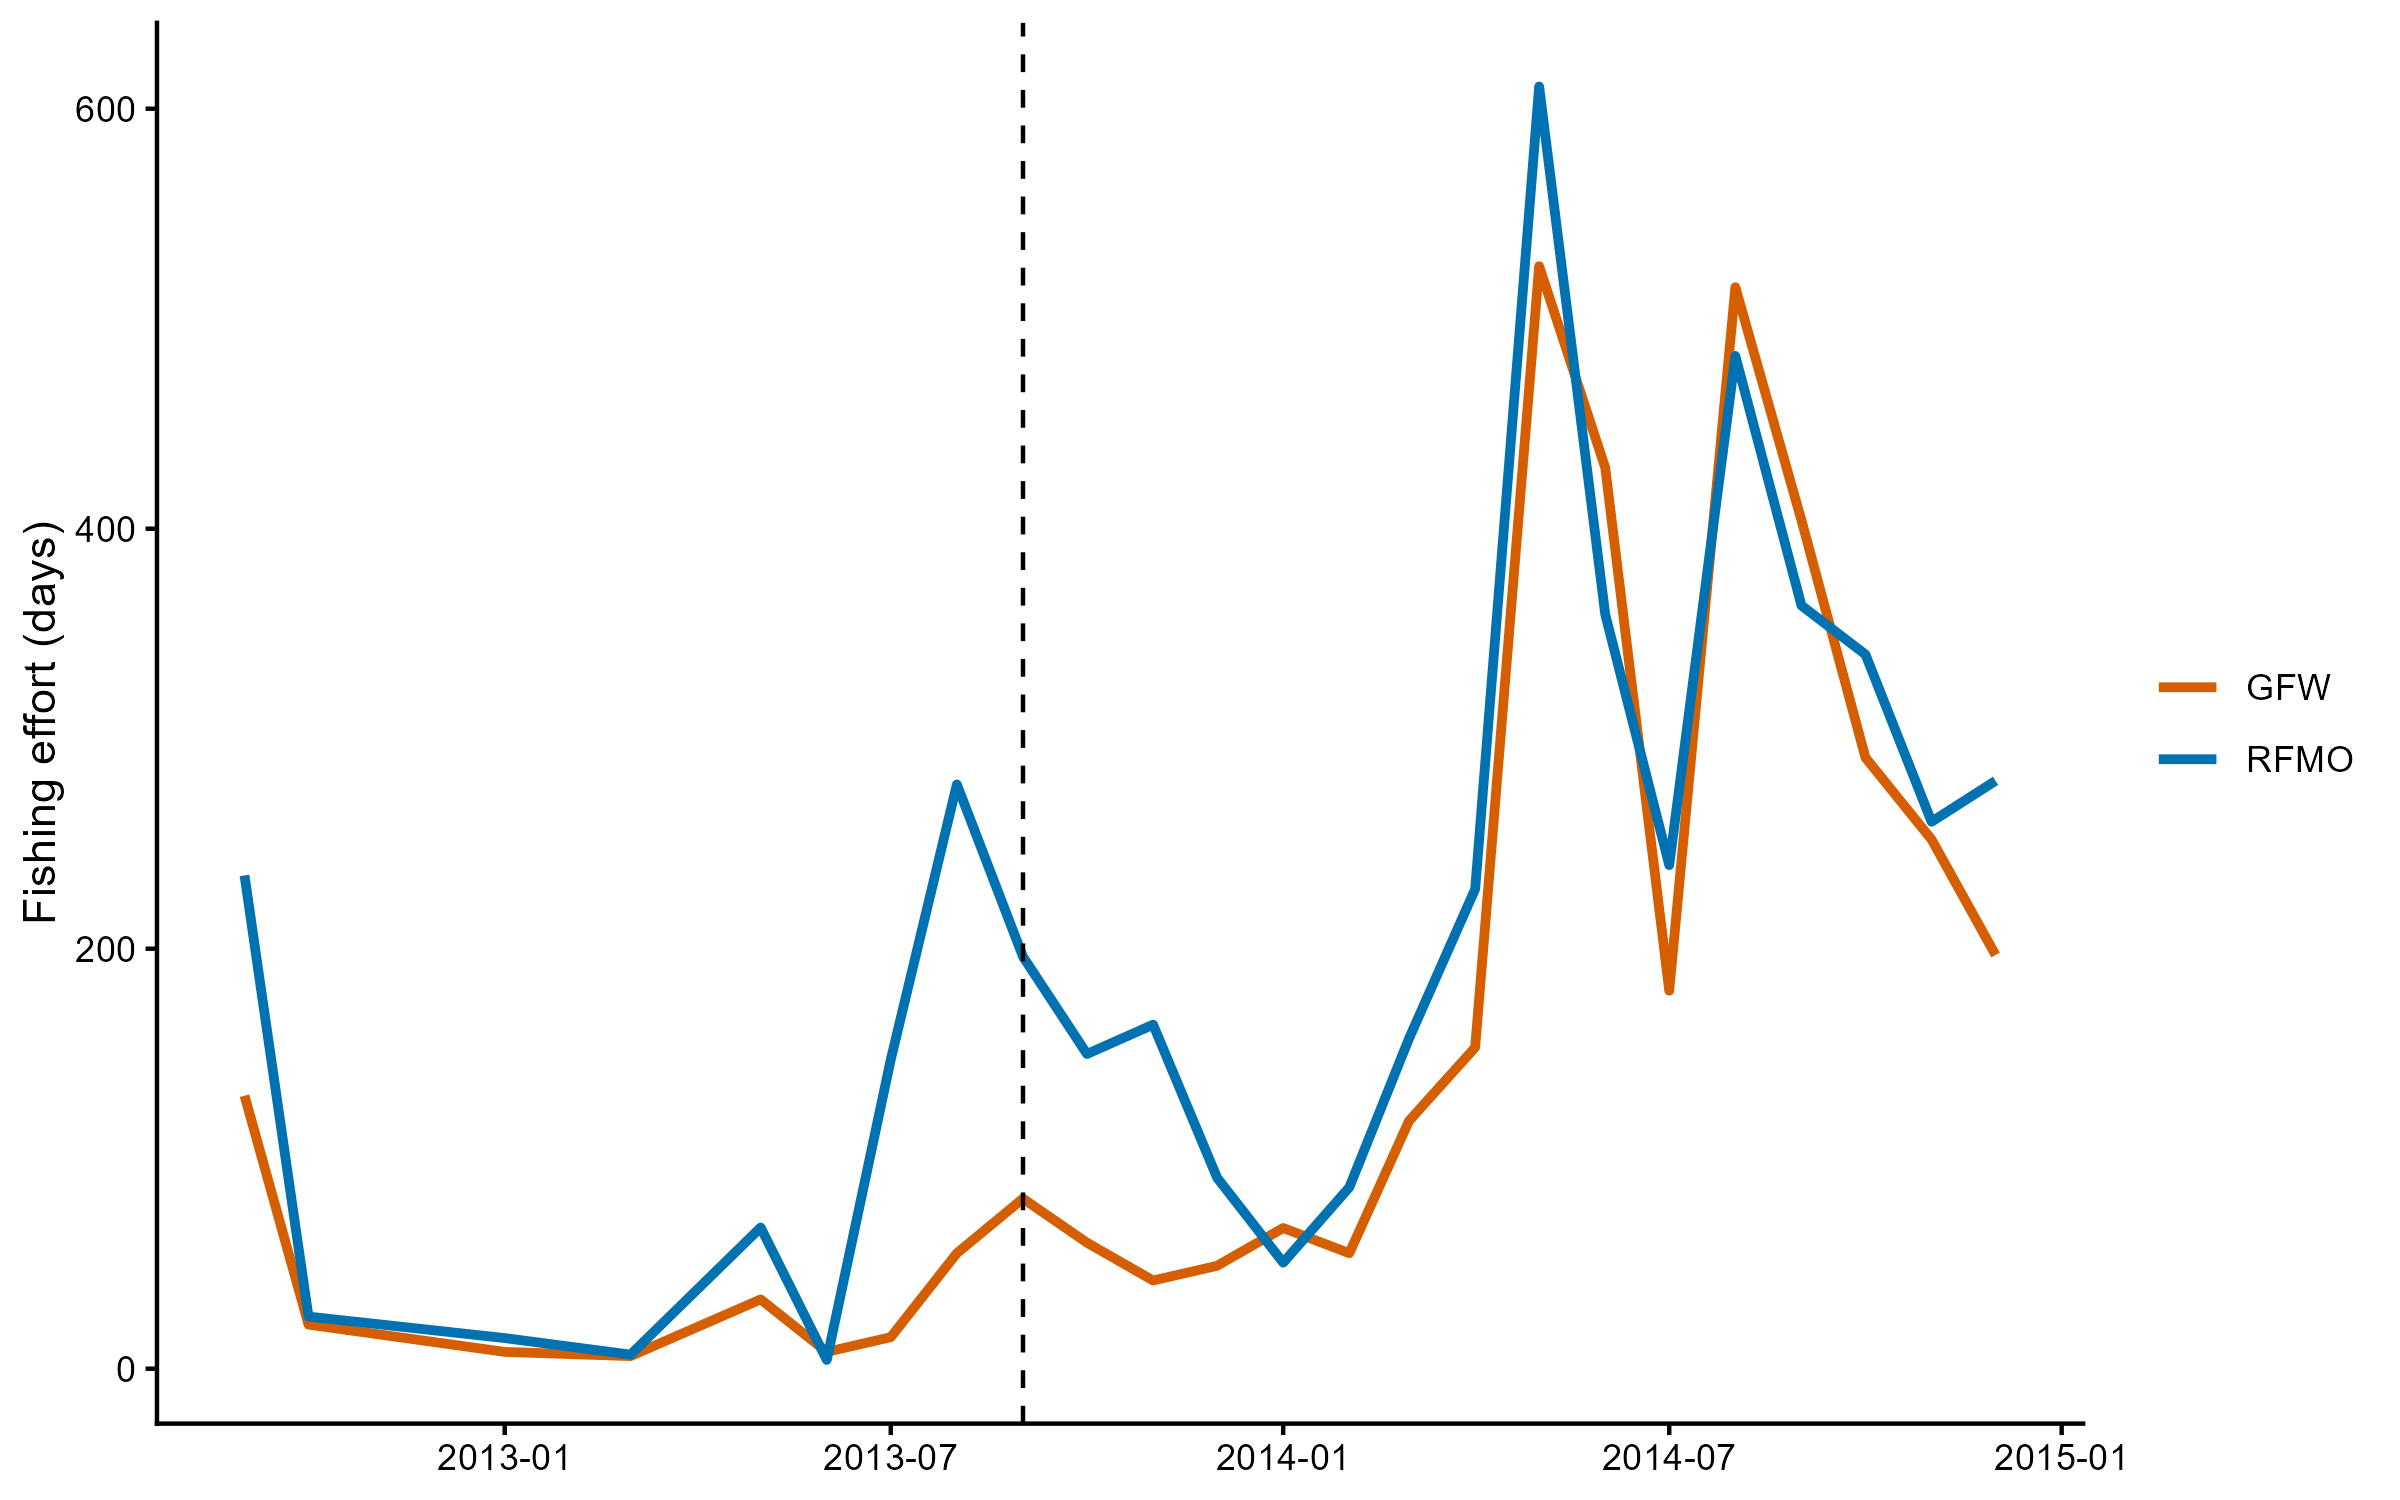
\includegraphics[keepaspectratio]{../results/figures/pipa_original/gfw_rfmo_days.png}}

}

\caption[Comparison of GFW daily effort and RFMO daily effort in
PIPA]{\label{fig-pipa-gfw-rfmo-days}Monthly fishing effort within the
Phoenix Islands Protected Area (PIPA) estimated from Regional Fisheries
Management Organization tuna purse seine data (Rodriguez and Juan Carlos
Villaseñor-Derbez (2026)) and Global Fishing Watch data (GFW) (Nate
Miller (he/him) et al. (2026)). Effort is expressed as days aggregated
across the entire PIPA region. Effort in days from GFW data is defined
as the number of unique vessel-specific fishing days per month. The
dashed vertical line marks the September 2013 announcement of PIPA.}

\end{figure}%

\begin{figure}

\centering{

\pandocbounded{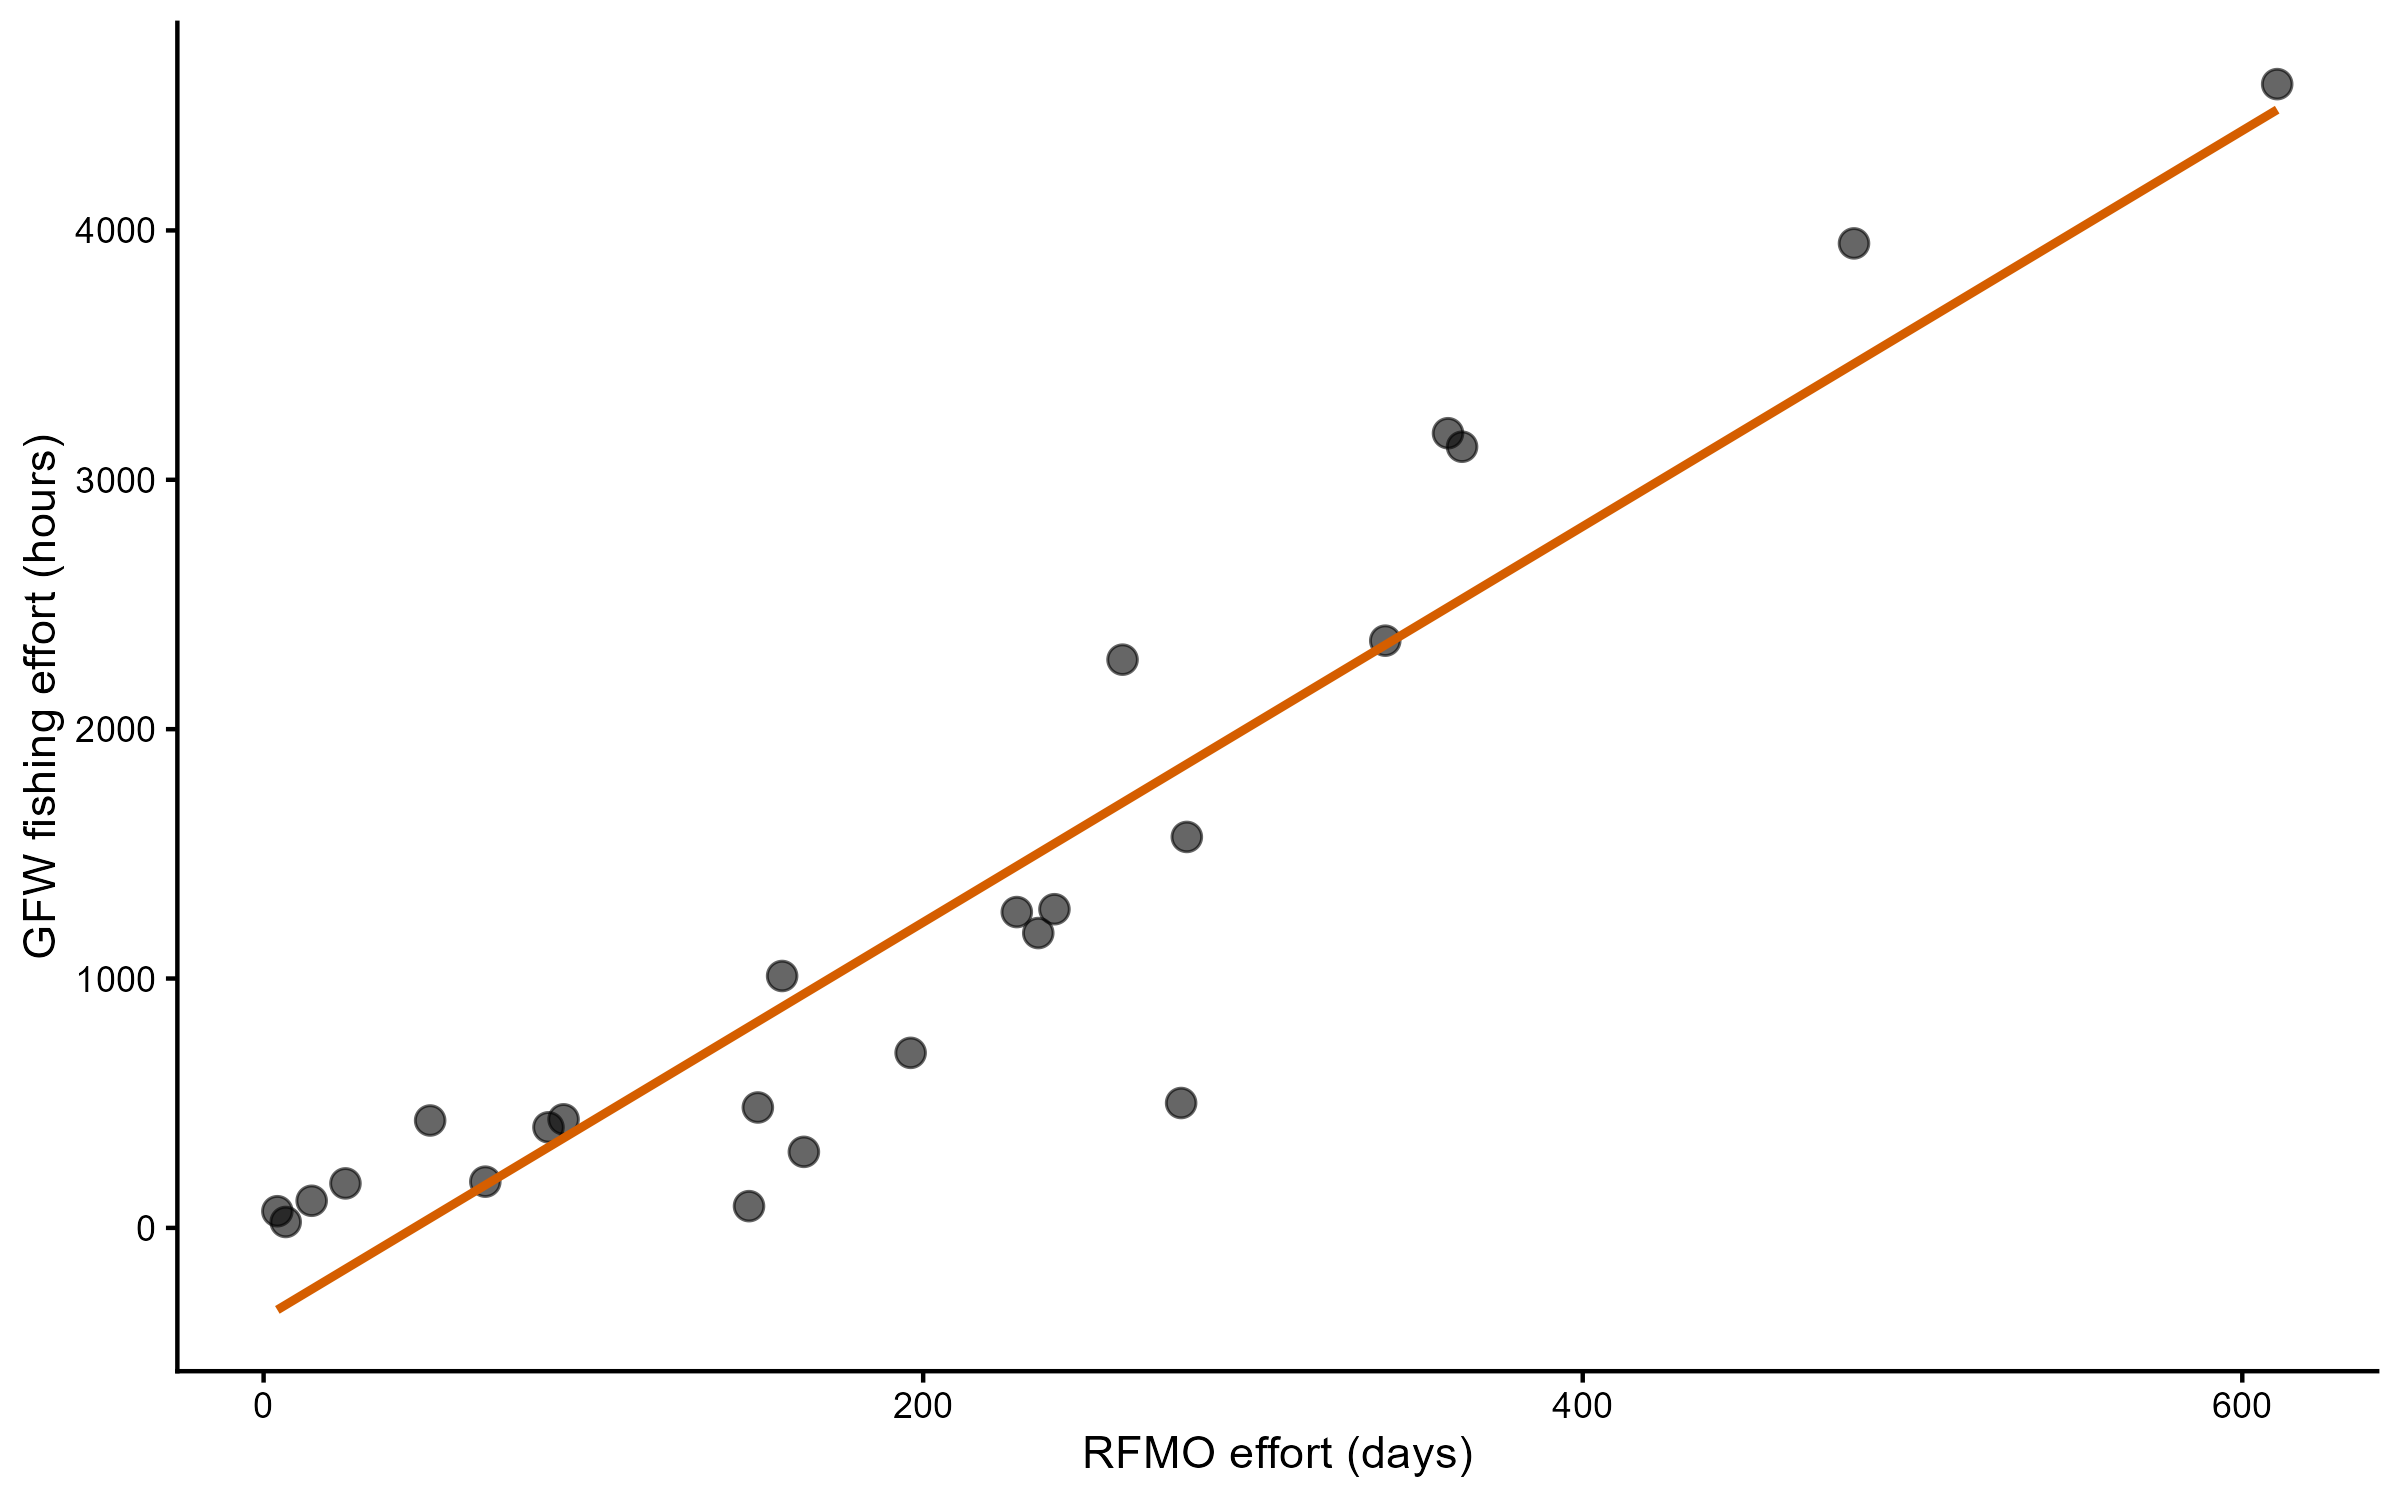
\includegraphics[keepaspectratio]{../results/figures/pipa_original/gfw_rfmo_days_v_hours.png}}

}

\caption[Comparison of GFW effort in hours to RFMO effort in
days]{\label{fig-pipa-gfw-rfmo-days-hours}Relationship between monthly
fishing effort estimates within the Phoenix Islands Protected Area
(PIPA) derived from Regional Fisheries Management Organization (RFMO)
tuna purse seine data (emilyrodriguezRFMOTunaCatch2026) and Global
Fishing Watch data (GFW) (Nate Miller (he/him) et al. (2026)). Each
points represents a month, with RFMO effort measured in fishing days and
GFW effort measured in fishing hours. The fitted linear regression line
illustrates the relationship between the two datasets.}

\end{figure}%

\begin{figure}

\centering{

\pandocbounded{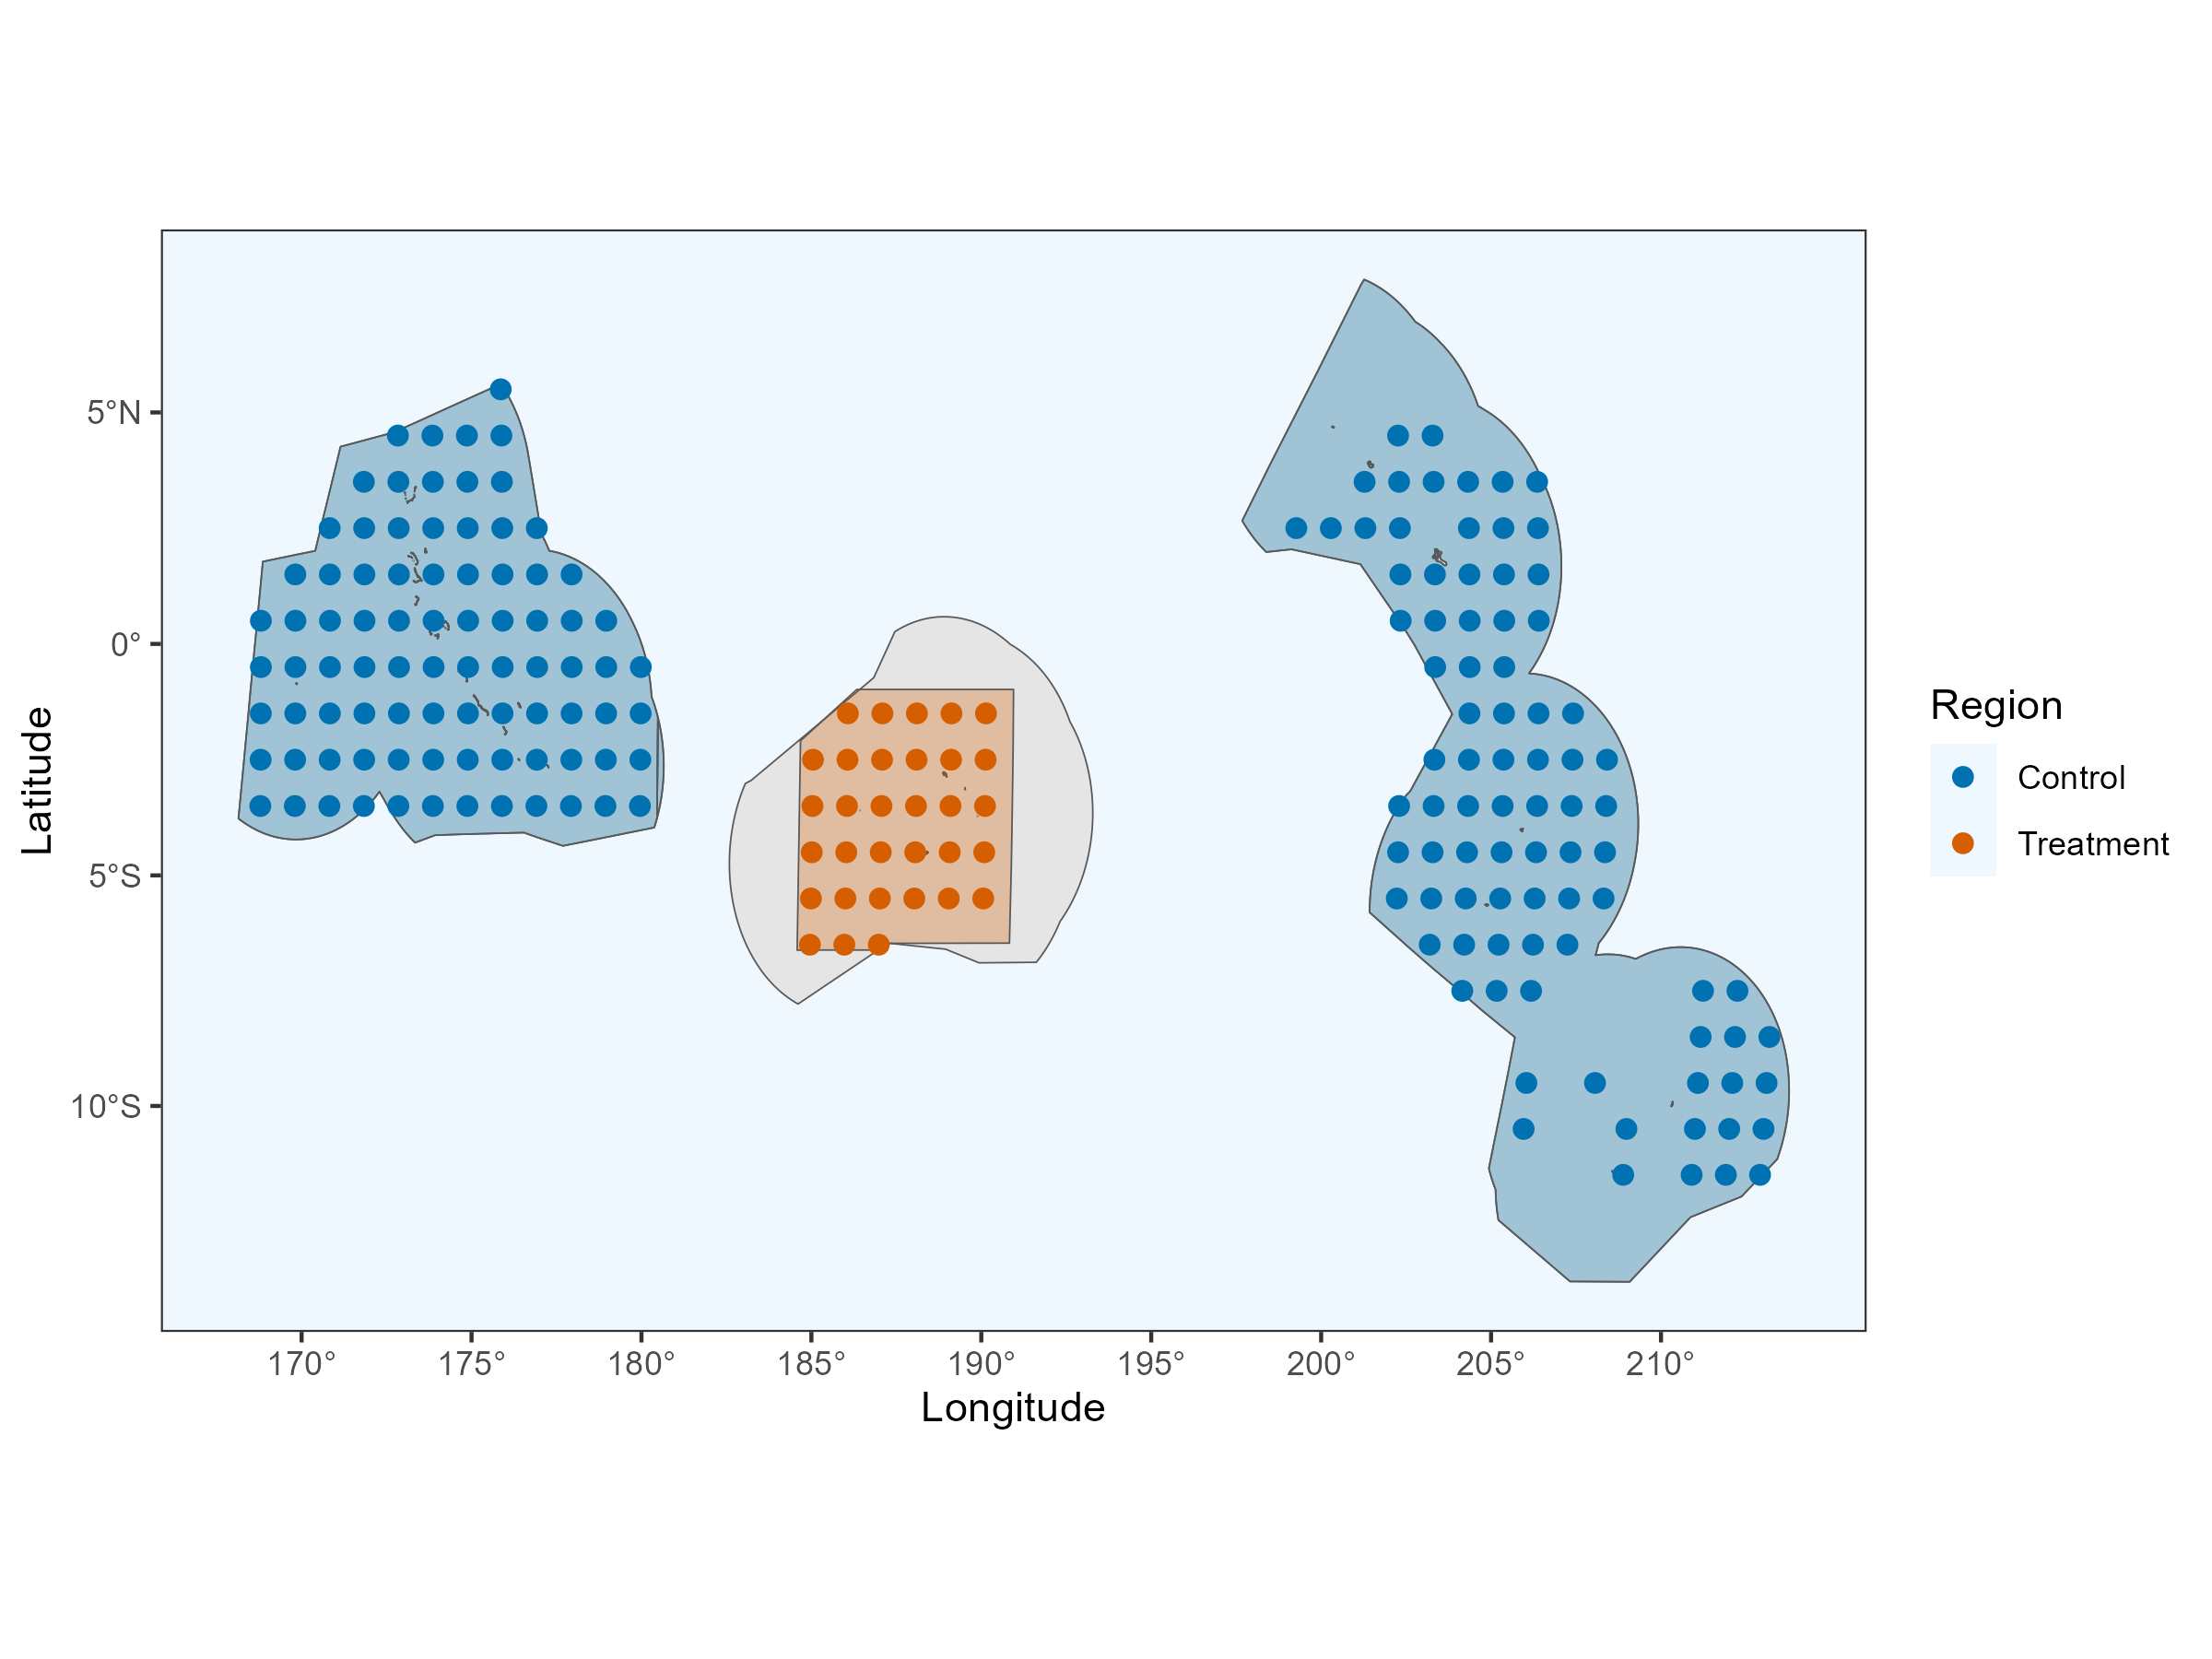
\includegraphics[keepaspectratio]{../results/figures/pipa_original/map_pipa.png}}

}

\caption[Phoenix Islands Protected Area and control
regions]{\label{fig-pipa-map}Spatial distribution of treated and control
regions used in Kiribati. The map shows the boundaries of the treated
(Phoenix Islands Protected Area) and control (Line and Gilbert Islands
exclusive economic zones) regions. Points indicate the centroids of the
1\(^\circ\) × 1\(^\circ\) grid cells included in the analysis. Nearby
exclusive economic zones are outlined.}

\end{figure}%

\begin{table}

\caption{\label{tbl-pipa-region_robust}Log-linear BACI regression
estimates at the region-level for Phoenix Islands Protected Area,
filtering for cells strictly inside PIPA. The interaction term estimates
the percentage change in the treatment region relative to the control
region during the anticipation period.}

\centering{

\centering
\begin{talltblr}[         %% tabularray outer open
entry=none,label=none,
note{}={+ p \num{< 0.1}, * p \num{< 0.05}, ** p \num{< 0.01}, *** p \num{< 0.001}},
]                     %% tabularray outer close
{                     %% tabularray inner open
width={1\linewidth},
colspec={X[]X[]X[]X[]X[]X[]},
hline{2}={1-6}{solid, black, 0.05em},
hline{10}={1-6}{solid, black, 0.05em},
hline{1}={1-6}{solid, black, 0.08em},
hline{13}={1-6}{solid, black, 0.08em},
column{2-6}={}{halign=c},
column{1}={}{halign=l},
}                     %% tabularray inner close
& log Effort (days) / 10,000 km² & log Effort (sets) / 10,000 km² & log Total Catch (kg) / 10,000 km² & CPUE (kg/day) & CPUE (kg/set) \\
(Intercept) & \num{-0.553} & \num{-0.583} & \num{9.665}*** & \num{10.218}*** & \num{10.248}*** \\
& (\num{0.336}) & (\num{0.368}) & (\num{0.374}) & (\num{0.116}) & (\num{0.111}) \\
treatment & \num{0.026} & \num{0.005} & \num{0.165} & \num{0.138} & \num{0.159} \\
& (\num{0.554}) & (\num{0.607}) & (\num{0.616}) & (\num{0.191}) & (\num{0.183}) \\
post & \num{1.218}** & \num{1.371}** & \num{1.330}** & \num{0.112} & \num{-0.041} \\
& (\num{0.445}) & (\num{0.487}) & (\num{0.494}) & (\num{0.153}) & (\num{0.147}) \\
treatment × post & \num{0.234} & \num{0.258} & \num{0.295} & \num{0.060} & \num{0.037} \\
& (\num{0.690}) & (\num{0.756}) & (\num{0.767}) & (\num{0.238}) & (\num{0.228}) \\
Num.Obs. & \num{51} & \num{51} & \num{51} & \num{51} & \num{51} \\
R2 & \num{0.256} & \num{0.264} & \num{0.266} & \num{0.085} & \num{0.057} \\
R2 Adj. & \num{0.208} & \num{0.217} & \num{0.220} & \num{0.027} & \num{-0.003} \\
\end{talltblr}

}

\end{table}%

\begin{figure}

\centering{

\pandocbounded{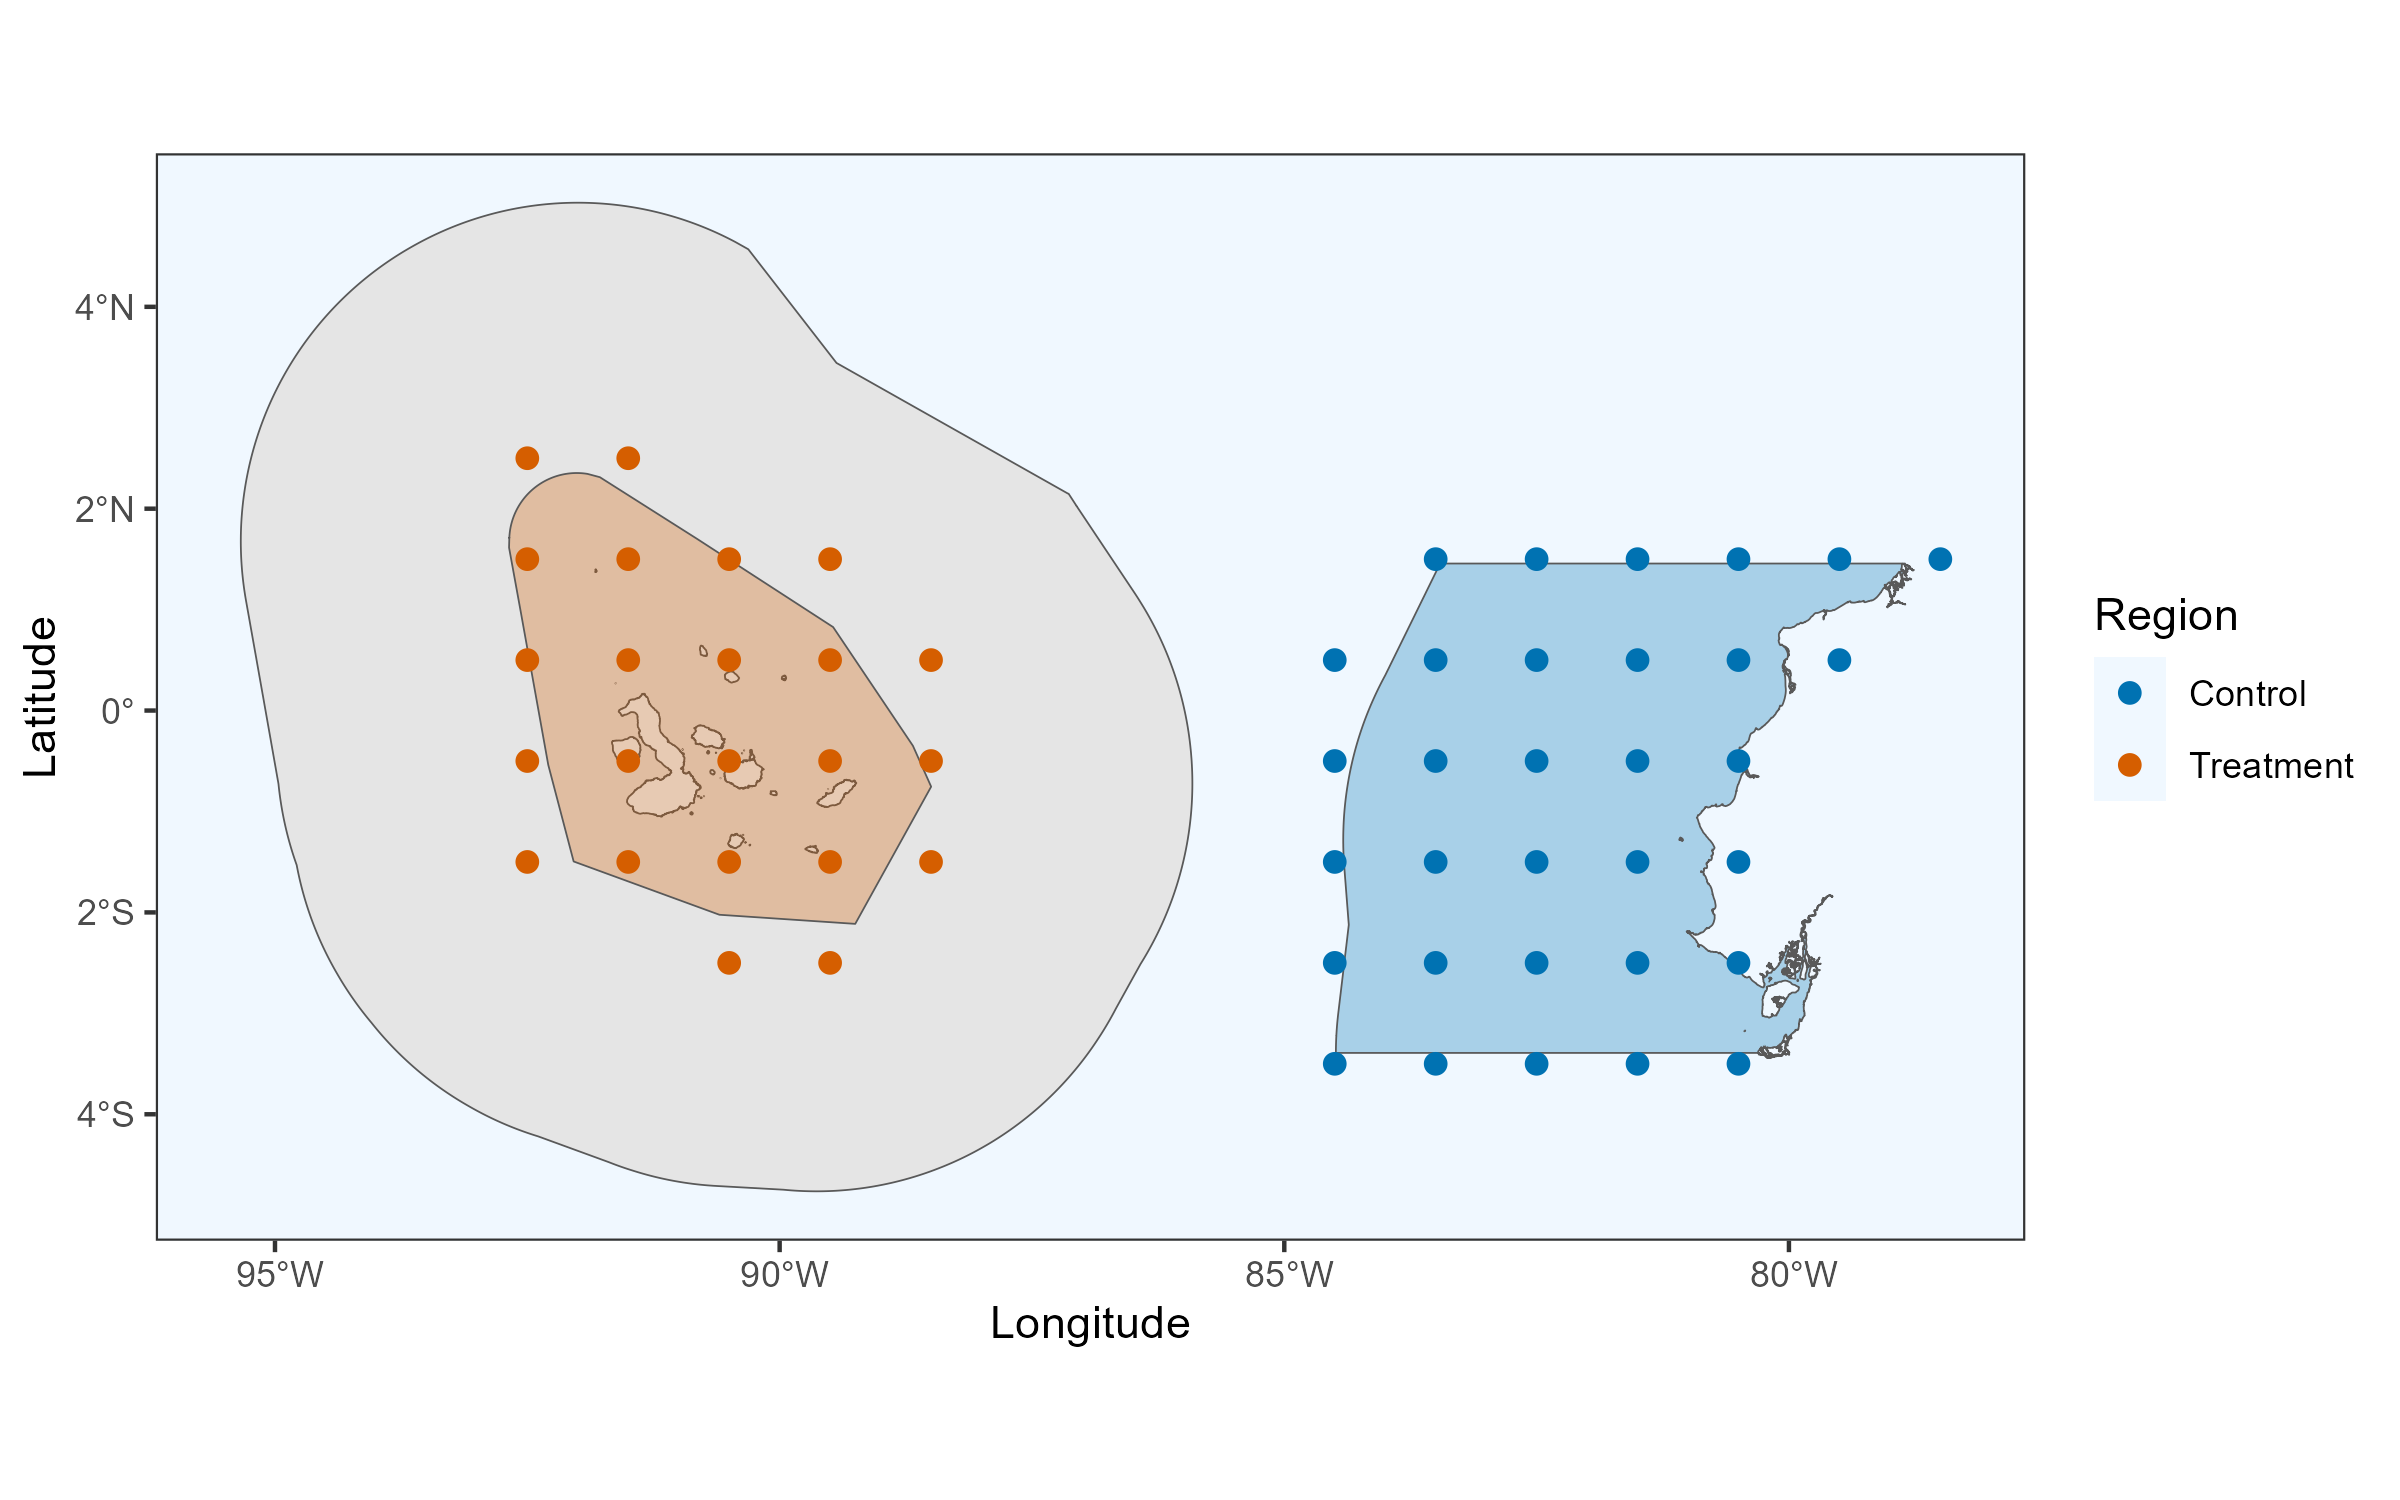
\includegraphics[keepaspectratio]{../results/figures/gmr/gmr_map.png}}

}

\caption[Galápagos Marine Reserve and control
region]{\label{fig-gmr-map}Spatial distribution of treated and control
regions used in Ecuador. The map shows the boundaries of the treated
(Galápagos Marine Reserve) and control (Ecuador mainland exclusive
economic zone) regions. Points indicate the centroids of the 1\(^\circ\)
× 1\(^\circ\) grid cells included in the analysis. Nearby exclusive
economic zones are outlined.}

\end{figure}%

\begin{figure}

\centering{

\pandocbounded{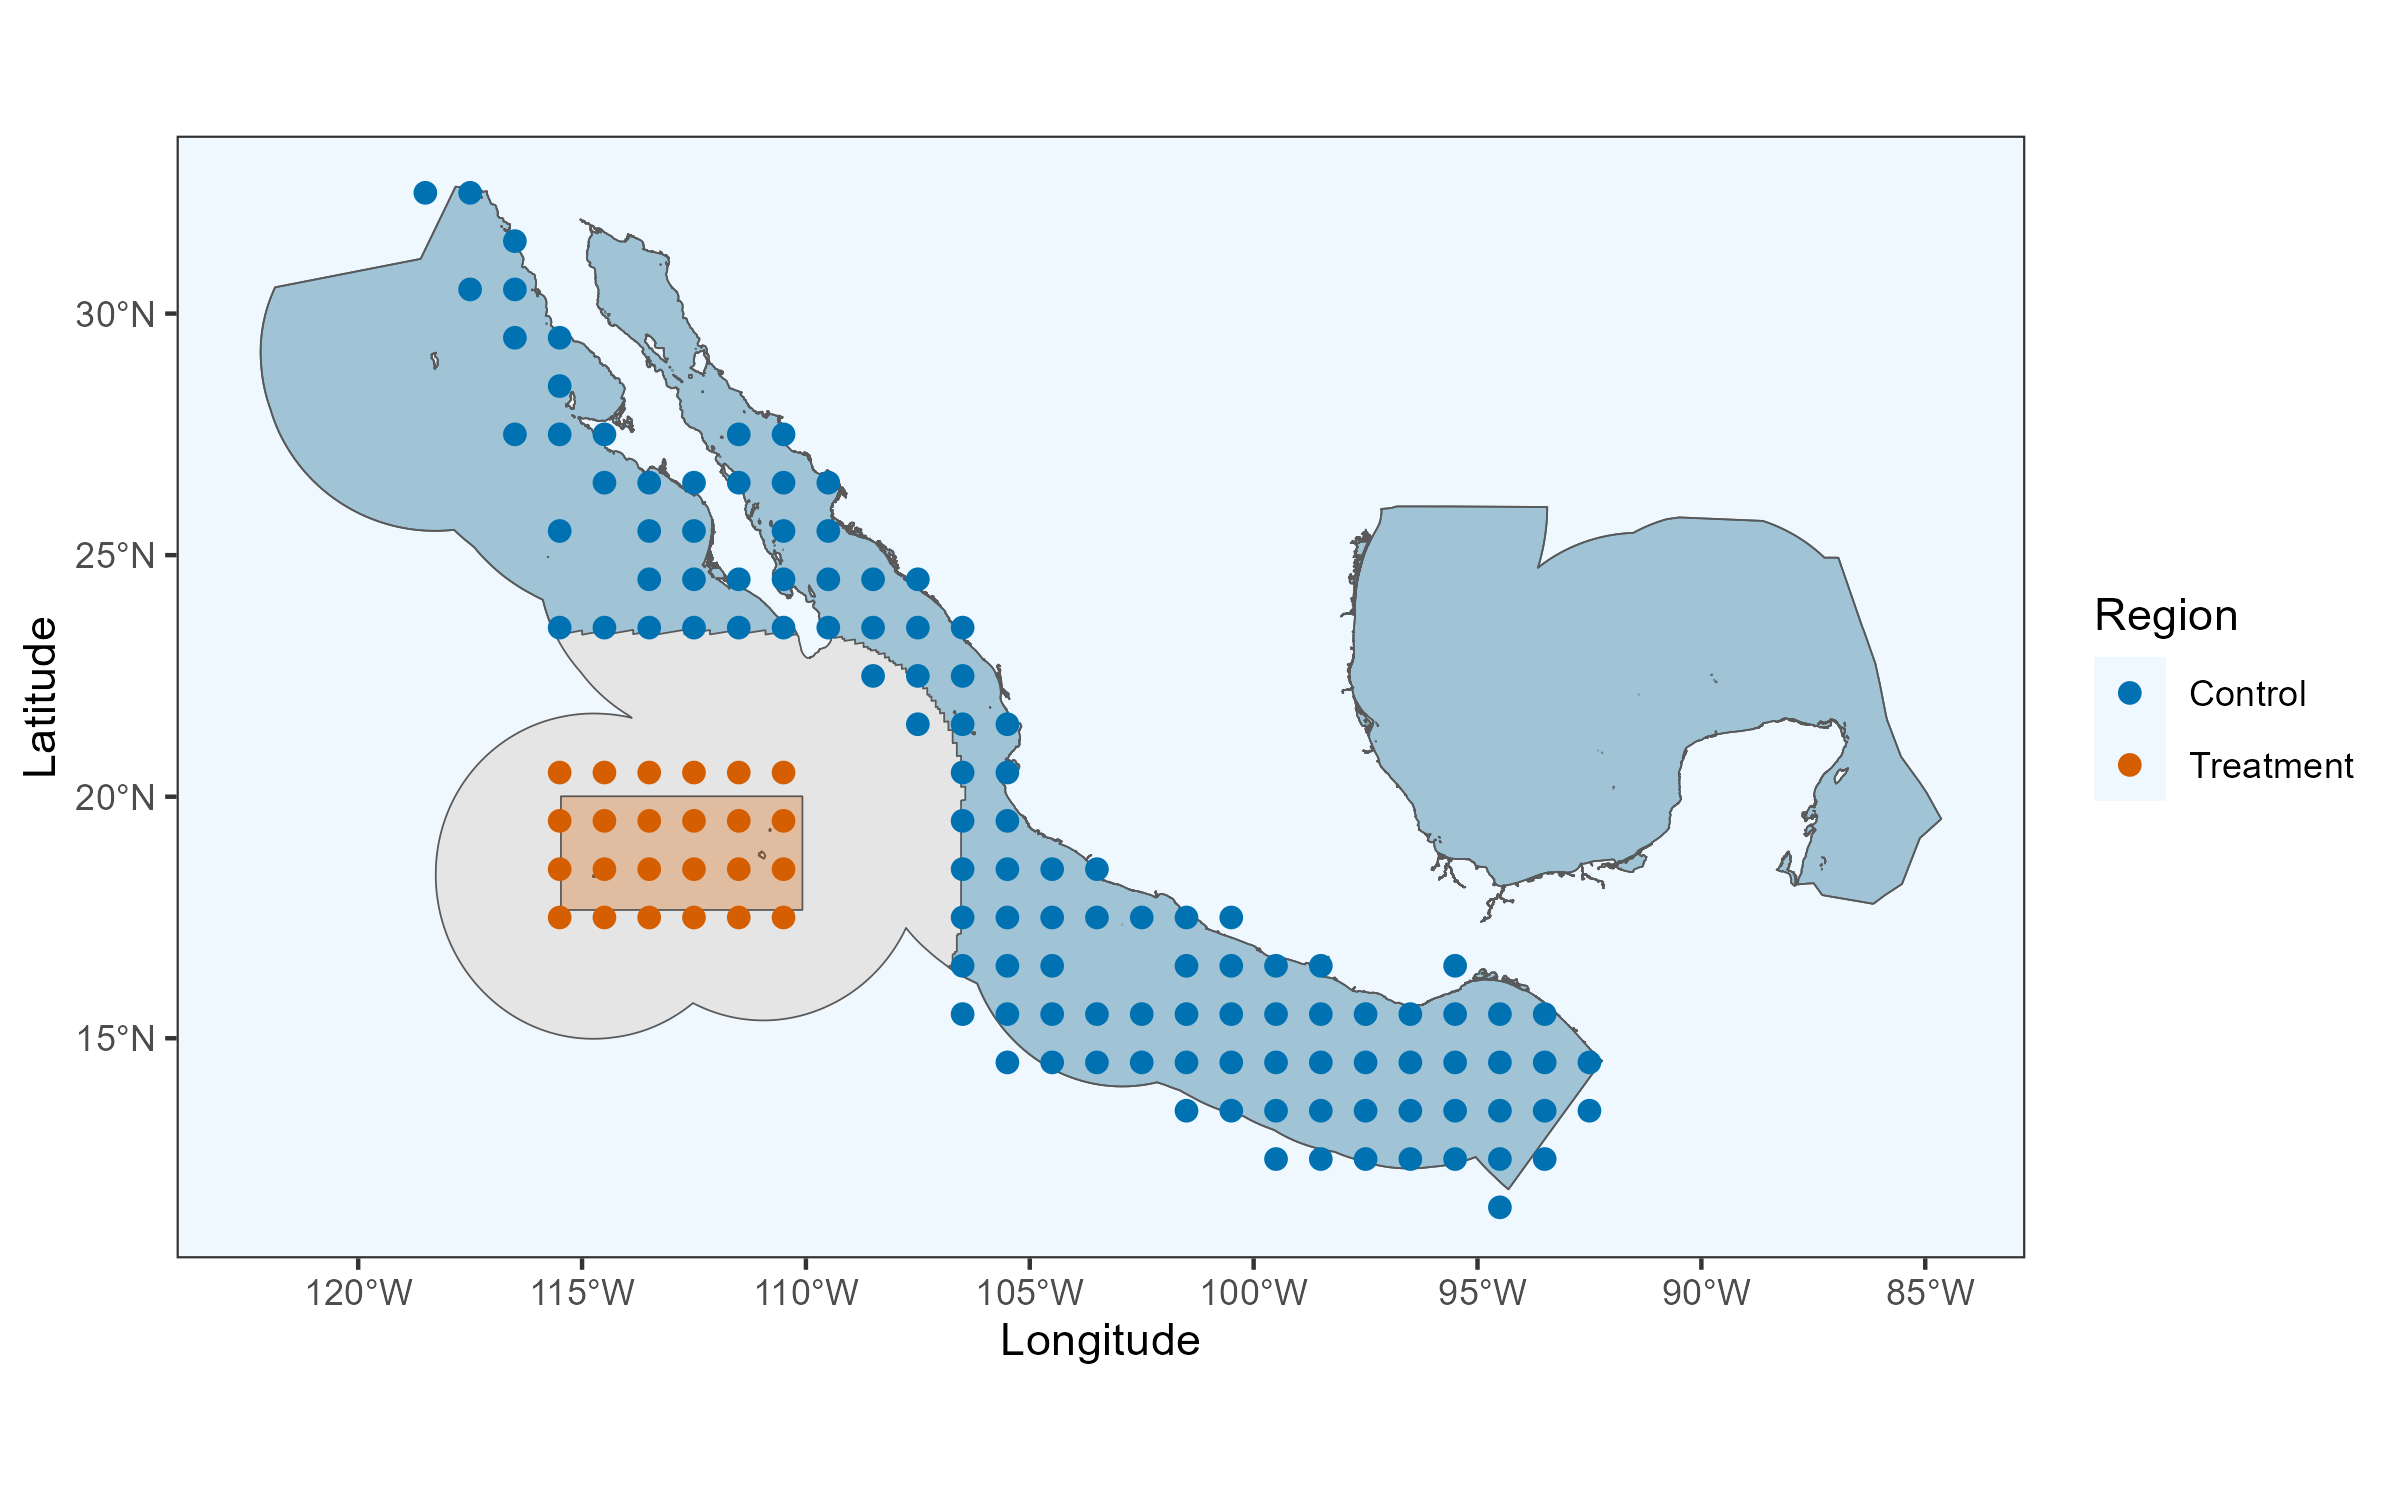
\includegraphics[keepaspectratio]{../results/figures/revilla/revilla_map.png}}

}

\caption[Revillagigedo National Park and control
region]{\label{fig-revilla-map}Spatial distribution of treated and
control regions used in Mexico. The map shows the boundaries of the
treated (Revillagigedo National Park) and control (Mexico exclusive
economic zone 200 nautical miles away from the national park) regions.
Points indicate the centroids of the 1\(^\circ\) × 1\(^\circ\) grid
cells included in the analysis. Nearby exclusive economic zones are
outlined.}

\end{figure}%

\begin{figure}

\centering{

\pandocbounded{\includegraphics[keepaspectratio]{../results/figures/revilla/cubic_timeseries_panels_region.png}}

}

\caption[Temporal trends in fishing effort, catch, and CPUE in
Revillagigedo National Park]{\label{fig-revilla-region}Cubic spline
estimates of temporal trends in three outcomes of interest for control
and treatment regions in the Revillagigedo National Park (RNP) at the
region-month level. Panels show observed monthly values (points) and
fitted cubic spline trajectories (lines) with shaded ribbons indicating
±1 standard error around the predicted values for (A) effort
(sets/10,000 km\(^2\)), (B) total catch (kg/10,000 km\(^2\), and (C)
CPUE (kg/sets) from Ocotber 2016 to November 2017. Panel D shows the
treatment (RNP) and control region. The vertical line indicates the
announcement of RNP (2017-10-05). Data include all observations prior to
implementation on 2017-11-27, with no post-implementation observations.}

\end{figure}%

\begin{table}

\caption{\label{tbl-revilla-region}Log-linear BACI regression estimates
at the region-level for Revillagigedo National Park. The interaction
term estimates the percentage change in the treatment region relative to
the control region during the anticipation period.}

\centering{

\centering
\begin{talltblr}[         %% tabularray outer open
entry=none,label=none,
note{}={+ p \num{< 0.1}, * p \num{< 0.05}, ** p \num{< 0.01}, *** p \num{< 0.001}},
]                     %% tabularray outer close
{                     %% tabularray inner open
width={1\linewidth},
colspec={X[]X[]X[]X[]},
hline{2}={1-4}{solid, black, 0.05em},
hline{10}={1-4}{solid, black, 0.05em},
hline{1}={1-4}{solid, black, 0.08em},
hline{13}={1-4}{solid, black, 0.08em},
column{2-4}={}{halign=c},
column{1}={}{halign=l},
}                     %% tabularray inner close
& log Effort (sets) / 10,000 km² & log Total Catch (kg) / 10,000 km² & CPUE (kg/set) \\
(Intercept) & \num{-0.358} & \num{8.808}*** & \num{9.166}*** \\
& (\num{0.294}) & (\num{0.349}) & (\num{0.104}) \\
treatment & \num{1.175}** & \num{0.994}+ & \num{-0.180} \\
& (\num{0.416}) & (\num{0.494}) & (\num{0.148}) \\
post & \num{-0.926} & \num{-0.613} & \num{0.313} \\
& (\num{1.062}) & (\num{1.259}) & (\num{0.376}) \\
treatment × post & \num{0.244} & \num{-0.017} & \num{-0.261} \\
& (\num{1.502}) & (\num{1.781}) & (\num{0.532}) \\
Num.Obs. & \num{26} & \num{26} & \num{26} \\
R2 & \num{0.314} & \num{0.181} & \num{0.110} \\
R2 Adj. & \num{0.220} & \num{0.070} & \num{-0.012} \\
\end{talltblr}

}

\end{table}%

\begin{figure}

\centering{

\pandocbounded{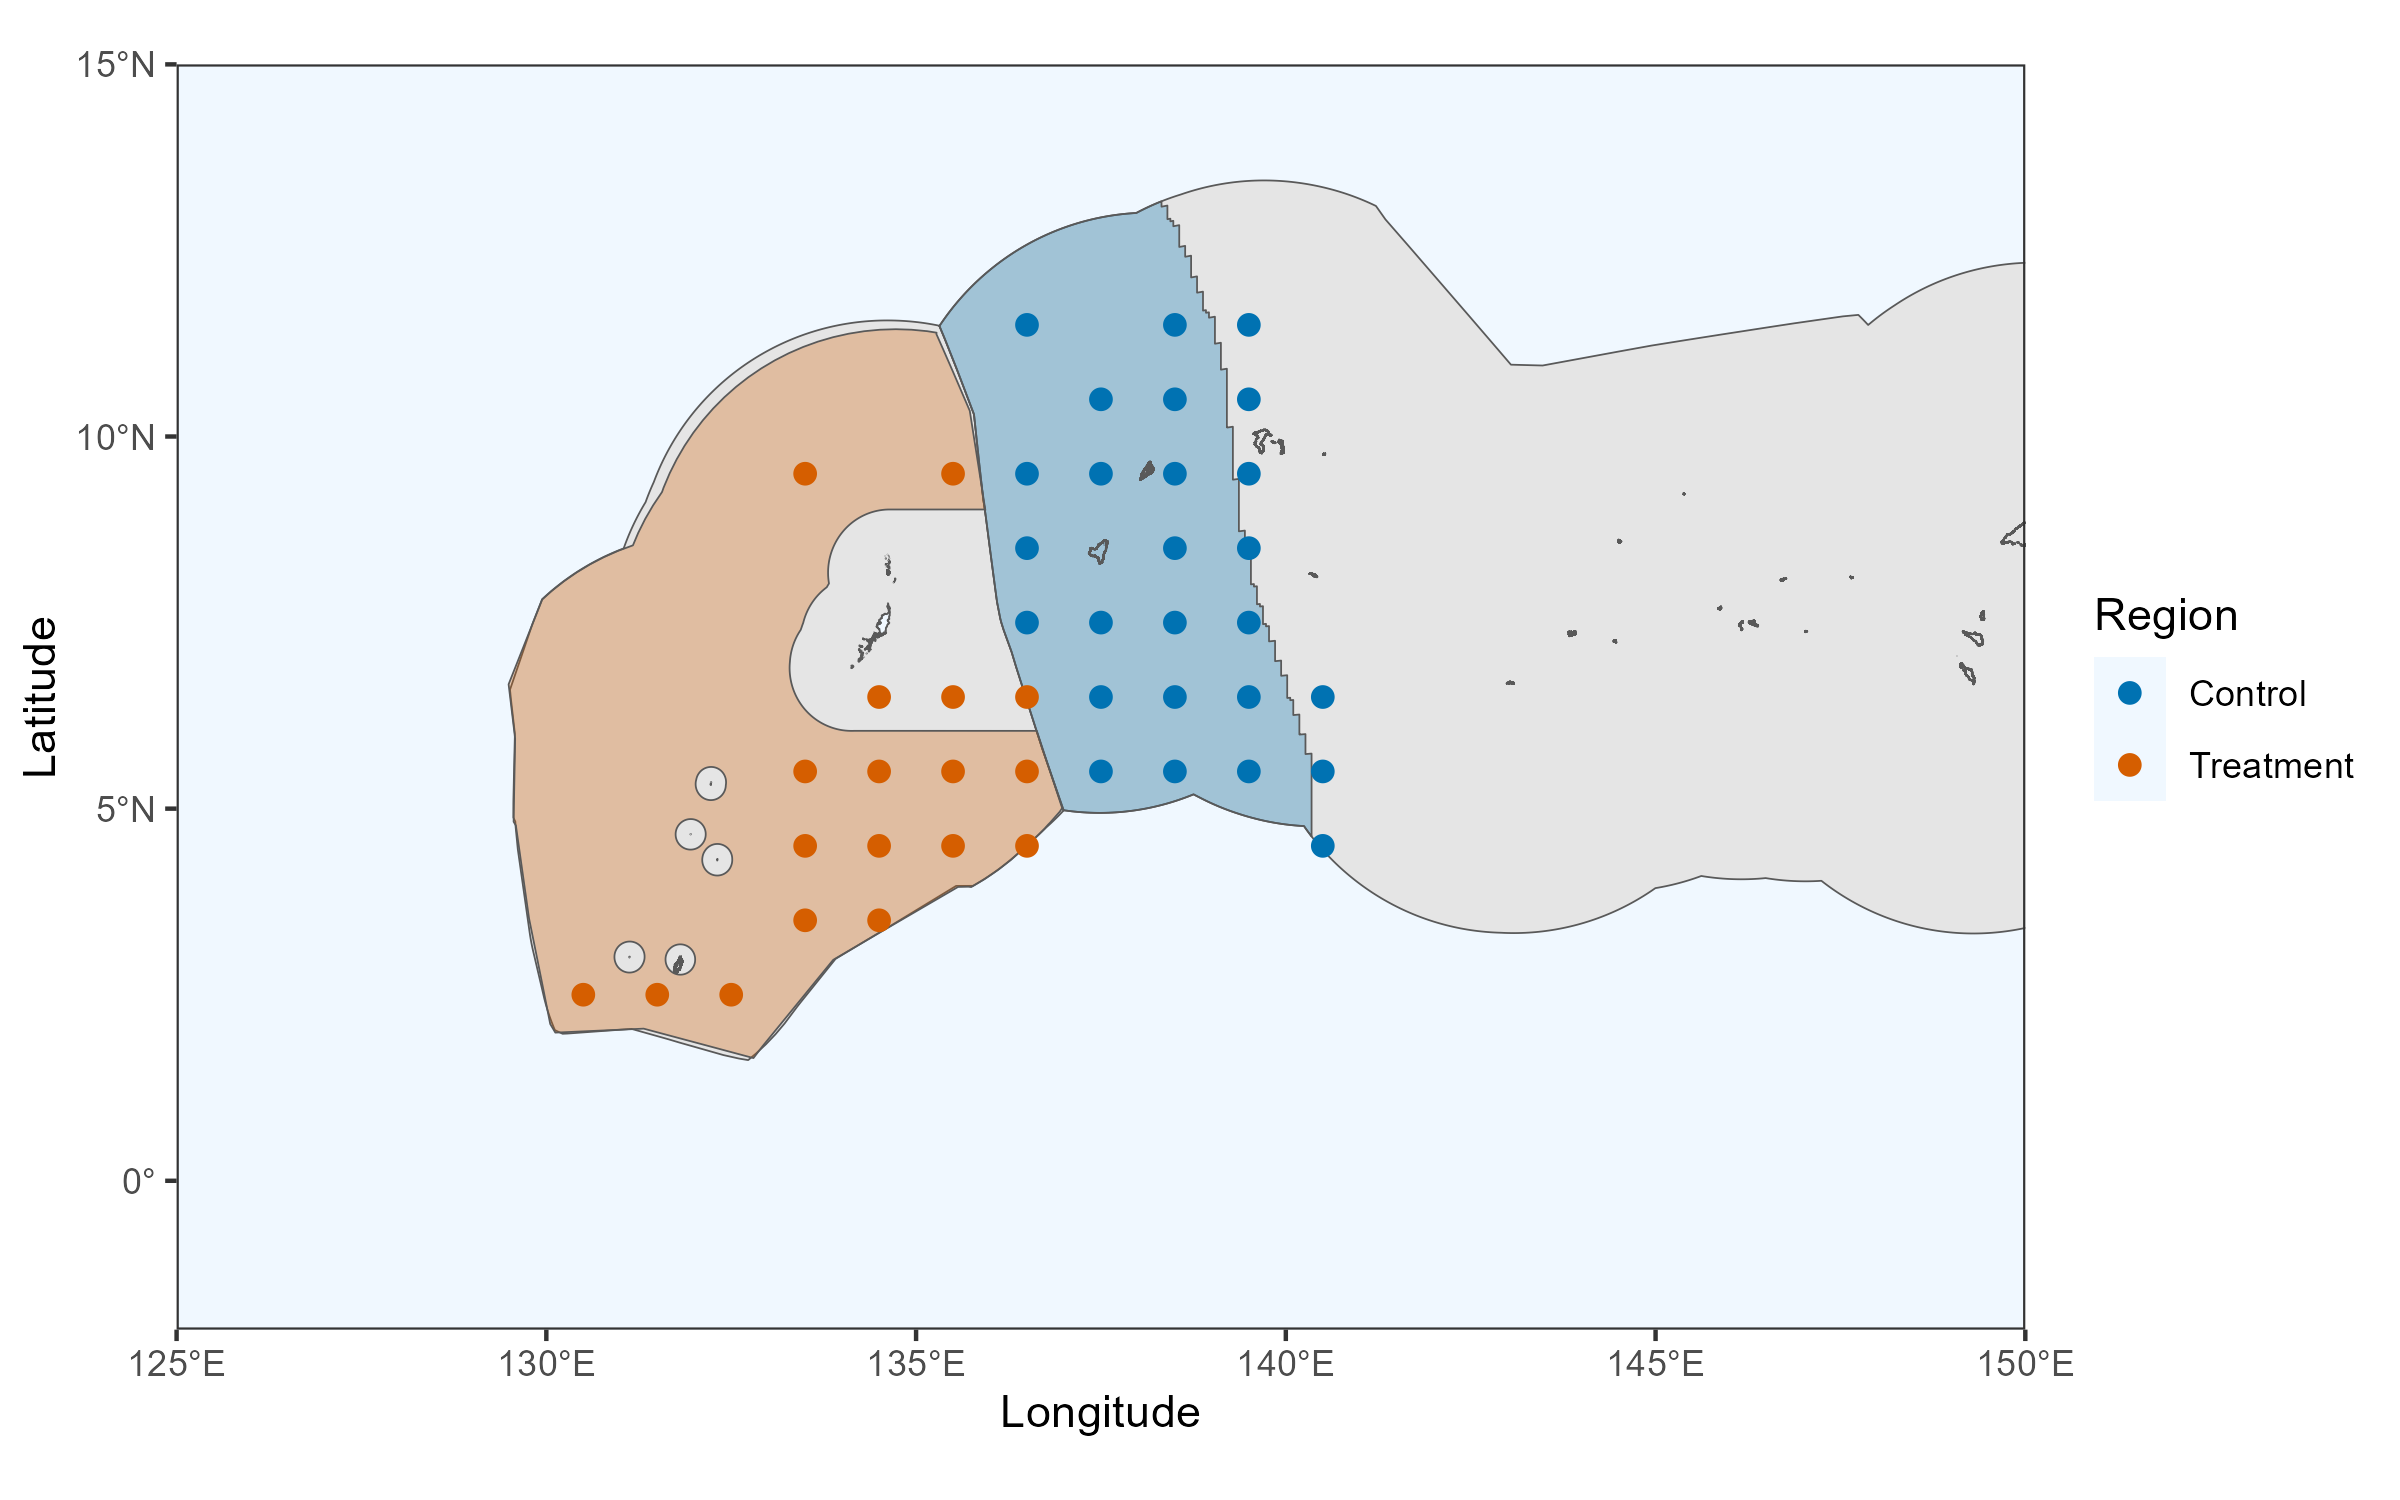
\includegraphics[keepaspectratio]{../results/figures/palau/palau_map.png}}

}

\caption[Palau National Marine Sanctuary and control
region]{\label{fig-palau-map}Spatial distribution of treated and control
regions used in Palau. The map shows the boundaries of the treated
(Palau National Marine Sanctuary) and control (Federated States of
Micronesia Exclusive Economic Zone within 200 nautical miles of Palau)
regions. Points indicate the centroids of the 1\(^\circ\) × 1\(^\circ\)
grid cells included in the analysis. Nearby exclusive economic zones are
outlined.}

\end{figure}%

\begin{figure}

\centering{

\pandocbounded{\includegraphics[keepaspectratio]{../results/figures/palau/cubic_timeseries_panels_region.png}}

}

\caption[Temporal trends in fishing effort, catch, and CPUE in Palau
National Marine Sanctuary]{\label{fig-palau-region}Cubic spline
estimates of temporal trends in five outcomes of interest for control
and treatment regions in the Palau National Marine Sanctuary (PNMS) at
the region-month level. Panels show observed monthly values (points) and
fitted cubic spline trajectories (lines) with shaded ribbons indicating
±1 standard error around the predicted values for (A) effort
(days/10,000 km\(^2\)), (B) effort (sets/10,000 km\(^2\)), (C) CPUE
(kg/day), (D) CPUE (kg/sets), and (E) total catch (kg/10,000 km\(^2\))
from October 2014 to December 2019. Panel F shows the treatment (PNMS)
and control regions. The vertical line indicates the announcement of
PNMS (2015-10-22). Data include all observations prior to MPA
implementation on 2020-01-01, with no post-implementation observations.}

\end{figure}%

\begin{table}

\caption{\label{tbl-palau-region}Log-linear BACI regression estimates at
the region-level for Palau National Marine Sanctuary The interaction
term estimates the percentage change in the treatment region relative to
the control region during the anticipation period.}

\centering{

\centering
\begin{talltblr}[         %% tabularray outer open
entry=none,label=none,
note{}={+ p \num{< 0.1}, * p \num{< 0.05}, ** p \num{< 0.01}, *** p \num{< 0.001}},
]                     %% tabularray outer close
{                     %% tabularray inner open
width={1\linewidth},
colspec={X[]X[]X[]X[]X[]X[]},
hline{2}={1-6}{solid, black, 0.05em},
hline{8}={1-6}{solid, black, 0.05em},
hline{1}={1-6}{solid, black, 0.08em},
hline{11}={1-6}{solid, black, 0.08em},
column{2-6}={}{halign=c},
column{1}={}{halign=l},
}                     %% tabularray inner close
& log Effort (days) / 10,000 km² & log Effort (sets) / 10,000 km² & log Total Catch (kg) / 10,000 km² & CPUE (kg/day) & CPUE (kg/set) \\
(Intercept) & \num{-1.007} & \num{-0.602} & \num{9.593}*** & \num{10.601}*** & \num{10.195}*** \\
& (\num{1.034}) & (\num{1.121}) & (\num{1.138}) & (\num{0.408}) & (\num{0.431}) \\
treatment & \num{-1.492}** & \num{-1.530}** & \num{-1.542}** & \num{-0.049} & \num{-0.012} \\
& (\num{0.417}) & (\num{0.452}) & (\num{0.459}) & (\num{0.164}) & (\num{0.174}) \\
post & \num{1.512} & \num{1.307} & \num{1.295} & \num{-0.217} & \num{-0.012} \\
& (\num{1.066}) & (\num{1.156}) & (\num{1.173}) & (\num{0.420}) & (\num{0.444}) \\
Num.Obs. & \num{27} & \num{27} & \num{27} & \num{27} & \num{27} \\
R2 & \num{0.362} & \num{0.331} & \num{0.327} & \num{0.017} & \num{0.000} \\
R2 Adj. & \num{0.309} & \num{0.275} & \num{0.271} & \num{-0.065} & \num{-0.083} \\
\end{talltblr}

}

\end{table}%

\subsection{Difference figures}\label{difference-figures}

\subsubsection{need to verify SE and add treatment/control
key}\label{need-to-verify-se-and-add-treatmentcontrol-key}

\begin{figure}

\centering{

\pandocbounded{\includegraphics[keepaspectratio]{../results/figures/pipa_original/differences.png fig-scap="Pre-implementation treatment-control differences in fishing effort, CPUE, and catch for PIPA"}}

}

\caption{\label{fig-differences-pipa}Temporal differences between
treatment and control regions for the Phoenix Islands Protected Area
(PIPA) in fishing activity and catch metrics prior to implementation.
Panels show spline-based estimates of the difference between treatment
and control regions (treatment minus control) for (A) effort
(days/10,000 km\(^2\)), (B) effort (sets/10,000 km\(^2\)), (C) CPUE
(kg/day), (D) CPUE (kg/sets), and (E) total catch (kg/10,000 km\(^2\))
from October 2014 to December 2019. The shaded ribbon represents ±1
standard error around the estimated treatment-control difference. Panel
F shows the treatment (PIPA) and control regions. The vertical line
indicates the announcement of PIPA (2013-09-01). Data include all
observations prior to MPA implementation on 2015-01-01, with no
post-implementation observations.}

\end{figure}%

\begin{figure}

\centering{

\pandocbounded{\includegraphics[keepaspectratio]{../results/figures/gmr/differences.png fig-scap="Pre-implementation treatment-control differences in fishing effort, CPUE, and catch for GMR"}}

}

\caption{\label{fig-differences-gmr}Temporal differences between
treatment and control regions for Galápagos Marine Reserve (GMR) in
fishing activity and catch metrics prior to implementation. Panels show
spline-based estimates of the difference between treatment and control
regions (treatment minus control) (A) effort (sets/10,000 km\(^2\)), (B)
total catch (kg/10,000 km\(^2\), and (C) CPUE (kg/sets) from January
1997 to December 2001. The shaded ribbon represents ±1 standard error
around the estimated treatment-control difference. Panel D shows the
treatment (GMR) and control region. The vertical line indicates the
implementation of GMR (1998-03-18). Data include all observations prior
to enforcement implementation on 2002-01-01, with no post-implementation
observations.}

\end{figure}%

\begin{figure}

\centering{

\pandocbounded{\includegraphics[keepaspectratio]{../results/figures/revilla/differences.png fig-scap="Pre-implementation treatment-control differences in fishing effort, CPUE, and catch for RNP"}}

}

\caption{\label{fig-differences-rnp}Temporal differences between
treatment and control regions for Revillagigedo National Park (RNP) in
fishing activity and catch metrics prior to implementation. Panels show
spline-based estimates of the difference between treatment and control
regions (treatment minus control) (A) effort (sets/10,000 km\(^2\)), (B)
total catch (kg/10,000 km\(^2\), and (C) CPUE (kg/sets) from Ocotber
2016 to November 2017. The shaded ribbon represents ±1 standard error
around the estimated treatment-control difference. Panel D shows the
treatment (GMR) and control region. The vertical line indicates the
announcement of RNP (2017-10-05). Data include all observations prior to
implementation on 2017-11-27, with no post-implementation observations.}

\end{figure}%

\begin{figure}

\centering{

\pandocbounded{\includegraphics[keepaspectratio]{../results/figures/palau/differences.png fig-scap="Pre-implementation treatment-control differences in fishing effort, CPUE, and catch for PNMS"}}

}

\caption{\label{fig-differences-pnms}Temporal differences between
treatment and control regions for Palau National Marine Sanctuary (PNMS)
in fishing activity and catch metrics prior to implementation. Panels
show spline-based estimates of the difference between treatment and
control regions (treatment minus control) for (A) effort (days/10,000
km\(^2\)), (B) effort (sets/10,000 km\(^2\)), (C) CPUE (kg/day), (D)
CPUE (kg/sets), and (E) total catch (kg/10,000 km\(^2\)) from October
2014 to December 2019. The shaded ribbon represents ±1 standard error
around the estimated treatment-control difference. Panel F shows the
treatment (PNMS) and control regions. The vertical line indicates the
announcement of PNMS (2015-10-22). Data include all observations prior
to MPA implementation on 2020-01-01, with no post-implementation
observations.}

\end{figure}%




\end{document}
